\documentclass[a4paper,11pt]{article}
		\usepackage[utf8]{inputenc}
	\usepackage[italian]{babel}
	\usepackage{hyperref}	%Consente l'inserimento di \url
	\usepackage{booktabs}	%Utilità di abbellimento tabelle
	\usepackage{longtable}
	\usepackage{tabularx}
	%\usepackage{widetable}
	\usepackage{array}
	\usepackage{listings}
	\usepackage{graphicx}
	\usepackage{caption}
	\usepackage{fancyhdr}
	\newenvironment{fixpic}{}{} % [1]
	\usepackage[a4paper,top=3cm,bottom=3cm,left=2.5cm,right=2.5cm]{geometry}
	%******
	\usepackage{makeidx}
	\usepackage{textcomp}
	\usepackage{multirow}
	\usepackage{rotfloat}
	\usepackage{lastpage}
	\usepackage{array}
	\usepackage{float}
	% *************************************
	% QUI CODICE PER \SUBSUBSUBSECTION
	\usepackage{titlesec}
	\titleclass{\subsubsubsection}{straight}[\subsection]
	
	\newcounter{subsubsubsection}[subsubsection]
	\renewcommand\thesubsubsubsection{\thesubsubsection.\arabic{subsubsubsection}}
	\renewcommand\theparagraph{\thesubsubsubsection.\arabic{paragraph}} % optional; useful if paragraphs are to be numbered
	
	\titleformat{\subsubsubsection}
	  {\normalfont\normalsize\bfseries}{\thesubsubsubsection}{1em}{}
	\titlespacing*{\subsubsubsection}
	{0pt}{3.25ex plus 1ex minus .2ex}{1.5ex plus .2ex}
	
	\makeatletter
	\renewcommand\paragraph{\@startsection{paragraph}{5}{\z@}%
	  {3.25ex \@plus1ex \@minus.2ex}%
	  {-1em}%
	  {\normalfont\normalsize\bfseries}}
	\renewcommand\subparagraph{\@startsection{subparagraph}{6}{\parindent}%
	  {3.25ex \@plus1ex \@minus .2ex}%
	  {-1em}%
	  {\normalfont\normalsize\bfseries}}
	\def\toclevel@subsubsubsection{4}
	\def\toclevel@paragraph{5}
	\def\toclevel@paragraph{6}
	\def\l@subsubsubsection{\@dottedtocline{4}{7em}{4em}}
	\def\l@paragraph{\@dottedtocline{5}{10em}{5em}}
	\def\l@subparagraph{\@dottedtocline{6}{14em}{6em}}
	\makeatother
	
	\setcounter{secnumdepth}{4}
	\setcounter{tocdepth}{4}
	%FINE \SUBSUBSUBSECTION
	%****************************************
	%STYLE PER INSERIMENTO DEL CODICE
	\lstdefinestyle{style1}{
	  belowcaptionskip=1\baselineskip,
	  breaklines=true,
	  frame=L,
	  xleftmargin=\parindent,
	  language=Pascal,
	  showstringspaces=false,
	  basicstyle=\footnotesize\ttfamily,
	  keywordstyle=\bfseries\color{blue},
	  commentstyle=\itshape\color{blue},
	  identifierstyle=\color{blue},
	  stringstyle=\color{orange},
	}
	
	\lstdefinestyle{style2}{
	  belowcaptionskip=1\baselineskip,
	  frame=L,
	  xleftmargin=\parindent,
	  language=C,
	  basicstyle=\footnotesize\ttfamily,
	  commentstyle=\itshape\color{blue},
	}
	\lstset{style=style1}
	
	%FINE STYLE INSERIMENTO CODICE
	%*****************************************
	\usepackage[default]{cantarell} %% Use option "defaultsans" to use cantarell as sans serif only
	\usepackage[T1]{fontenc}        %% for font
	\hypersetup{colorlinks, linkcolor=black, urlcolor=blue}
	\newcommand{\addglos}{\begin{scriptsize}{\textbf{\ped{G}}} \end{scriptsize}} 
	\pagestyle{fancy}
	\fancyhead{}
	\fancyfoot{}
	%\fancyhead[L]{
\includegraphics[scale=0.28]{team_not_found.jpeg}}
	\fancyhead[L]{
\includegraphics[scale=0.15]{../../team404_small.jpg} \hspace{2mm} QUIZZIPEDIA}
	\fancyhead[R]{\leftmark}
	\fancyfoot[L]{Universit\`a degli studi di Padova - IS 2015/2016 \\ \url{team404swe@gmail.com}}

	
	%Commando usato per la tabella di informazioni sul documento
	\newcommand{\introtab}[9]{
		\begin{table}[ht]
		\begin{center}		
		\begin{tabular}{r l}			
			\toprule		
			\multicolumn{2}{c}{\textbf{ Informazioni sul documento }} \\
			\midrule 
			\textbf{Nome Documento}			& \vline \hspace{3.5 mm} {#1} \\
			\textbf{Versione}				& \vline \hspace{3.5 mm} {#2} \\
			\textbf{Uso} 					& \vline \hspace{3.5 mm} {#3} \\
			\textbf{Data Creazione} 		& \vline \hspace{3.5 mm} {#4} \\
			\textbf{Data Ultima Modifica} 	& \vline \hspace{3.5 mm} {#5} \\
			\textbf{Redazione}				& \vline \hspace{3.5 mm} {#6} \\
											%& \vline \hspace{3.5 mm} {#7} \\	
			\textbf{Verifica} 				& \vline \hspace{3.5 mm} {#7}	\\
			\textbf{Approvazione}			& \vline \hspace{3.5 mm} {#8}\\	
			\textbf{Committente} 			& \vline \hspace{3.5 mm} Zucchetti SPA\\
			\textbf{Lista di distribuzione} & \vline \hspace{3.5 mm} Prof. Vardanega Tullio \\														& \vline \hspace{3.5 mm} TEAM404 \\
	\bottomrule	
	\end{tabular}
	\end{center}
	\end{table}
	}
	% Comando di inizio del registro
	\newcommand{\beginregistro}{
		%\begin{longtable}{{|p{0.10\textwidth}|p{0.20\textwidth}|p{0.15\textwidth}|p{0.50\textwidth}|}}
		\begin{longtable}{{|p{1.5cm}|p{2.5cm}|p{2cm}|p{8cm}|}} 
	 		\hline	
	}
	% commando usato pr inserire una riga al registro delle modifiche
	\newcommand{\rigaregistro}[4]{
		{\footnotesize #1} & {\footnotesize #2} &  {\footnotesize #3} &  {\footnotesize #4} \\
			\hline	
	}
	% Comando di fine registro
	\newcommand{\fineregistro}{ \end{longtable}	}
	
	%************************************************
	% commandi per il GLOSSARIO
	%***********************************************
	% Commando di inizio tabella Glossario
	\newcommand{\beginglos}{
		\begin{longtable}{{p{0.20\textwidth}p{0.65\textwidth}}}	
	}
	% Commando per i termini del glossario
	
	\newcommand{\itemglos}[2]{
		\textbf{#1 :} & {#2} \\ \\ \\
	}
	% Commando fine Glossario
	\newcommand{\fineglos}{ \end{longtable} }
	% Comando per aggiungere una ssezione numerata con lettere al glossario
	\newcommand{\sezione}{
	\subsection{}	
	\rule[0.3pt]{\linewidth}{0.4pt} \\ % Linea orizzontale
	}
	
\newcommand{\sezioneglos}[1] { 
  \newpage
  \cleardoublepage
  \phantomsection
  \addcontentsline{toc}{section}{#1}
  \vspace{11pt}
  \textbf{\huge{#1} } % Lettera grande 
  \\
  \rule[0.3pt]{\linewidth}{0.4pt} \\ % Linea orizzontale
  \fancyhead[R]{#1}
}
	\newcommand{\code}[1]{\texttt{#1}}

	\title{\textbf{{\fontsize{8mm}{5mm}\selectfont QUIZZIPEDIA}}}
	\date{}
	\author{}	


\begin{document}
	\maketitle
	\thispagestyle{empty}
	\begin{center}	
	
\includegraphics{../team_not_found.jpg}\\
	\fontsize{5mm}{3mm}\url{team404swe@gmail.com}\\
	
	\vspace{50mm}
	\textbf{Definizione di Prodotto 1.0}
	\end{center}
	\introtab{Definizione di Prodotto}	%1 nome documento
			{1.0} 							%2 versione
			{Esterno} 						%3 Uso
			{20 maggio 2016} 				%4 Data cre
			{\today} 						%5 Data mod
			{D. Bortot}		%6 Redazione
			{Alex Beccaro } 			%7 Verifica
			{Martin V. Mbouenda} 				%8 Approvazione
	\newpage
	\thispagestyle{empty}
	\null  

	\newpage
	\newpage
	\fancyhead[R]{REGISTRO DELLE MODIFICHE}
	\fancyfoot[R]{\thepage}
	
	\hspace{30 mm}
	\section*{Registro delle modifiche}
	
	\beginregistro
	
	\rigaregistro{\textbf{Versione}}{\textbf{Autore}}{\textbf{Data}}		 {\hspace{5 mm}}
	\rigaregistro{0.0.4}{Luca Alessio (Analista)}{09/06/2016}{Stesura campi "Funzione del componente" e "Relazione con altri componenti" di tutti gli elementi.} 
	\rigaregistro{0.0.3}{Luca Alessio (Analista)}{08/06/2016}{Adattamento delle varie sezioni alle nuove indicazioni contenute nel documento riveduto specifica\_tecnica\_2.0.pdf (re-impaginazione dei paragrafi e revisione della struttura del documento).} 
	\rigaregistro{0.0.2}{Davide Bortot (Progettista)}{05/06/2016}{Impostata la struttura della sezioni "ViewModel", "View", "Model" e della sezione "Tracciamento".} 
	\rigaregistro{0.0.1}{Davide Bortot (Progettista)}{30/05/2016}{Creazione e impostazione documento. Definite sezioni "Sommario" e "Introduzione".}
	
	\fineregistro

	\newpage
	\fancyhead[R]{\leftmark}
	\tableofcontents
	\pagenumbering{Roman}
	\newpage
	\listoffigures
	\listoftables
	
	\newpage
	\pagenumbering{arabic}
	
	\section*{Sommario}
	Questo documento, redatto dal gruppo \textbf{Team404}, contiene la descrizione di dettaglio dell'architettura software sulla quale verrà sviluppato il progetto Quizzipedia, commissionato da Zucchetti S.p.A..
Le specifiche del documento si basano sull'architettura generale descritta nel documento "\textit{specifica\_tecnica\_2.0.pdf}".
	
	\newpage
	\section{Introduzione}
	\subsection{Scopo del documento}
	Il documento ha lo scopo di definire nel dettaglio la struttura del sistema Quizzipedia, approfondendone la descrizione già definita nel documento di Specifica Tecnica. Per ogni package del sistema verrà data una descrizione estensiva delle sue classiPer poter sviluppare al meglio il prodotto, i programmatori dovranno attenersi alle specifiche definite in questo documento.
	
	\subsection{Scopo del prodotto}
	Il progetto \textbf{Quizzipedia} ha come obiettivo lo sviluppo di un sistema software basato su tecnologie Web (Javascript\addglos, Node.js\addglos, HTML5\addglos, CSS3\addglos) che permetta la creazione, gestione e fruizione di questionari. Il sistema dovrà quindi poter archiviare i questionari suddivisi per argomento, le cui domande dovranno essere raccolte attraverso uno specifico linguaggio di markup (Quiz Markup Language) d'ora in poi denominato QML\addglos. In un caso d'uso a titolo esemplificativo, un "esaminatore" dovrà poter costruire il proprio questionario scegliendo tra le domande archiviate, ed il questionario così composto sarà presentato e fruibile all' "esaminando", traducendo l'oggetto QML in una pagina HTML\addglos, tramite un'apposita interfaccia web. Il sistema presentato dovrà inoltre poter proporre questionari preconfezionati e valutare le risposte fornite dall'utente finale.
	\\
	Per un'analisi più precisa ed approfondita del progetto si rimanda al documento\\ "\textit{analisi\_dei\_requisiti\_3.0.pdf}".
	\subsection{Glossario}
	Viene allegato un glossario nel file ``\textit{glossario\_3.0.pdf}'' nel quale viene data una definizione a tutti i termini che in questo documento appaiono con il simbolo '\addglos' a pedice.
	\subsection{Riferimenti}
		\subsubsection{Normativi}

		\begin{itemize}
			\item Capitolato d'appalto Quizzipedia:\\
			\url{http://www.math.unipd.it/~tullio/IS-1/2015/Progetto/C5.pdf}
			\item Norme di Progetto: "\textit{norme\_di\_progetto\_3.0.pdf}"
		\end{itemize}
		\subsubsection{Informativi}
		\begin{itemize}
			\item Corso di Ingegneria del Software anno 2015/2016:\\
			\url{http://www.math.unipd.it/~tullio/IS-1/2015/}
			\item Regole del progetto didattico:\\
			\url{http://www.math.unipd.it/~tullio/IS-1/2015/Dispense/PD01.pdf}
			\url{http://www.math.unipd.it/~tullio/IS-1/2015/Progetto/}\\
		\end{itemize}
	\pagebreak
	\newpage
	\section{Architettura generale}

	\newpage
	\section{Package View}
\begin{figure}[h!]
\begin{center}
	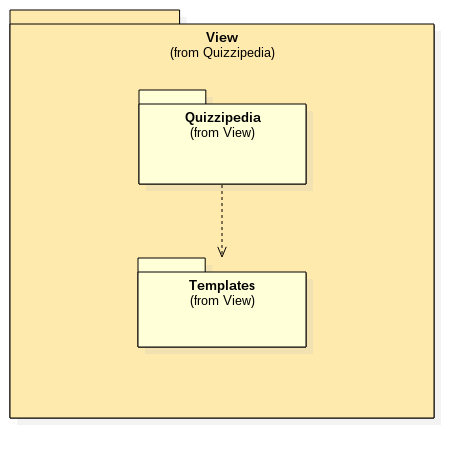
\includegraphics[scale=0.7]{../images/ViewPackage.png}
\end{center}
\end{figure}

\subsection{View::Pages}
\subsubsection{View::Pages::Page}
\begin{itemize}
\item\textbf{Funzione del componente:} rappresenta una pagina web
				\item\textbf{Relazioni d'uso con altre componenti:} L'interfaccia Page viene concretizzata dalle sue classi derivate, una rappresentativa per ogni pagina dell'applicazione\\ \\
\item\textbf{Attributi}:
	\begin{itemize}
		\item\code{- controller}: riferimento al controller della page\\
	\end{itemize}
\item\textbf{Metodi}:
	\begin{itemize}
		\item\code{+ show()}: metodo astratto che mostra il contenuto della pagina\\
	\end{itemize}
\end{itemize}

\subsubsection{View::Pages::LoginPage}
\begin{itemize}
\item\textbf{Funzione del componente:} visualizza il form di autenticazione e permette il login dell'utente. Fornisce inoltre un link alla pagina di registrazione e uno alla pagina di recupero della password 
				\item\textbf{Relazioni d'uso con altre componenti:} concretizza l'interfaccia Page da cui è diretta discendente e utilizza il template LoginForm\\ \\
La classe utilizza:
	\begin{itemize}
		\item View::Pages::Page\\
		\item View::Templates::LoginForm\\
	\end{itemize}
\item\textbf{Metodi}:
	\begin{itemize}
		\item\code{+ show()}: visualizza il form di autenticazione al sistema\\
		\textbf{Precondizioni}: viene richiesta la pagina di autenticazione. L'utente non è ancora autenticato\\
		\textbf{Postcondizioni}: viene visualizzata la pagina di autenticazione\\
	\end{itemize}
\end{itemize}

\subsubsection{View::Pages::RegistrationPage}
\begin{itemize}
\item\textbf{Funzione del componente:} visualizza il form di registrazione. Fornisce inoltre un link alla pagina di login
				\item\textbf{Relazioni d'uso con altre componenti:} concretizza l'interfaccia Page da cui è diretta discendente e utilizza il template RegistrationForm\\ \\
La classe utilizza:
	\begin{itemize}
		\item View::Pages::Page\\
		\item View::Templates::RegistrationForm\\
	\end{itemize}
\item\textbf{Metodi}:
	\begin{itemize}
		\item\code{+ show()}: visualizza il form di registrazione al sistema\\
		\textbf{Precondizioni}: viene richiesta la pagina di registrazione. L'utente non è autenticato\\
		\textbf{Postcondizioni}: viene visualizzata la pagina di registrazione\\
	\end{itemize}
\end{itemize}

\subsubsection{View::Pages::PasswordRecoveryPage}
\begin{itemize}
\item\textbf{Funzione del componente:} visualizza il form per il recupero della password
				\item\textbf{Relazioni d'uso con altre componenti:} concretizza l'interfaccia Page da cui è diretta discendente e utilizza il template PasswordRecoveryForm\\ \\
La classe utilizza:
	\begin{itemize}
		\item View::Pages::Page\\
		\item View::Templates::PasswordRecoveryForm\\
	\end{itemize}
\item\textbf{Metodi}:
	\begin{itemize}
		\item\code{+ show()}: visualizza il form per il recupero della password\\
		\textbf{Precondizioni}: viene richiesta la pagina della procedura per il recupero della password. L'utente non è autenticato\\
		\textbf{Postcondizioni}: viene visualizzata la pagina della procedura per il recupero della password\\
	\end{itemize}
\end{itemize}

\subsubsection{View::Pages::QuizCreationPage}
\begin{itemize}
\item\textbf{Funzione del componente:} visualizza il form di creazione di un nuovo questionario
				\item\textbf{Relazioni d'uso con altre componenti:} concretizza l'interfaccia Page da cui è diretta discendente e utilizza il template QuizCreationForm\\ \\
La classe utilizza:
	\begin{itemize}
		\item View::Pages::Page\\
		\item View::Templates::QuizCreationForm\\
	\end{itemize}
\item\textbf{Attributi}:
	\begin{itemize}
		\item\code{- user}: l'utente autenticato che sta creando il questionario\\
	\end{itemize}
\item\textbf{Metodi}:
	\begin{itemize}
		\item\code{+ show()}: visualizza il form per la creazione di un questionario\\
		\textbf{Precondizioni}: viene richiesta la pagina di creazione di un questionario. L'utente è autenticato\\
		\textbf{Postcondizioni}: viene visualizzata la pagina di creazione di un questionario\\
	\end{itemize}
\end{itemize}

\subsubsection{View::Pages::QuestionUpdatePage}
\begin{itemize}
\item\textbf{Funzione del componente:} visualizza il form di modifica di una domanda
				\item\textbf{Relazioni d'uso con altre componenti:} concretizza l'interfaccia Page da cui è diretta discendente e utilizza il template QuestionForm\\ \\
La classe utilizza:
	\begin{itemize}
		\item View::Pages::Page\\
		\item View::Templates::QuestionForm\\
	\end{itemize}
\item\textbf{Attributi}:
	\begin{itemize}
		\item\code{- user}: l'utente autenticato che sta modificando la domanda\\
		\item\code{- question}: la domanda da modificare\\
	\end{itemize}
\item\textbf{Metodi}:
	\begin{itemize}
		\item\code{+ show()}: visualizza il form per la modifica di una domanda compilato con i dati attuali\\
		\textbf{Precondizioni}: viene richiesta la pagina di modifica di una domanda. L'utente è autenticato\\
		\textbf{Postcondizioni}: viene visualizzata la pagina di modifica di una domanda\\
	\end{itemize}
\end{itemize}

\subsubsection{View::Pages::QuestionCreationPage}
\begin{itemize}
\item\textbf{Funzione del componente:} visualizza il form di creazione di una nuova domanda
				\item\textbf{Relazioni d'uso con altre componenti:} concretizza l'interfaccia Page da cui è diretta discendente e utilizza il template QuestionForm\\ \\
La classe utilizza:
	\begin{itemize}
		\item View::Pages::Page\\
		\item View::Templates::QuestionForm\\
	\end{itemize}
\item\textbf{Attributi}:
	\begin{itemize}
		\item\code{- user}: l'utente autenticato che sta creando la domanda\\
	\end{itemize}
\item\textbf{Metodi}:
	\begin{itemize}
		\item\code{+ show()}: visualizza il form per la creazione di una domanda\\
		\textbf{Precondizioni}: viene richiesta la pagina di creazione di una domanda. L'utente è autenticato\\
		\textbf{Postcondizioni}: viene visualizzata la pagina di creazione di una domanda\\
	\end{itemize}
\end{itemize}

\subsubsection{View::Pages::QuestionManagementPage}
\begin{itemize}
\item\textbf{Funzione del componente:} visualizza la lista delle domande create dall'utente
				\item\textbf{Relazioni d'uso con altre componenti:} concretizza l'interfaccia Page da cui è diretta discendente e utilizza il template QuestionList\\ \\
La classe utilizza:
	\begin{itemize}
		\item View::Pages::Page\\
		\item View::Templates::QuestionList\\
		\item View::Templates::Question\\
	\end{itemize}
\item\textbf{Attributi}:
	\begin{itemize}
		\item\code{- user}: l'utente autenticato che sta gestendo le proprie domande\\
		\item\code{- questions}: le domande dell'utente user\\
	\end{itemize}
\item\textbf{Metodi}:
	\begin{itemize}
		\item\code{+ show()}: visualizza la lista delle domande dell'utente permettendone la modifica e l'eliminazione. Permette inoltre di creare una nuova domanda, di ordinare la lista e fare una ricerca tra le domande\\
			\textbf{Precondizioni}: viene richiesta la pagina di gestione delle proprie domande. L'utente è autenticato\\
			\textbf{Postcondizioni}: viene visualizzata la pagina di gestione delle proprie domande\\
		\item\code{+ sort()}: ordina la lista delle domande secondo il criterio \code{by}\\
			\textbf{Precondizioni}: l'utente ha selezionato un criterio di ordinamento\\
			\textbf{Postcondizioni}: la lista di domande viene ordinata secondo il criterio inserito\\
			\textbf{Parametri}:
				\begin{itemize}
					\item\code{by}: criterio di ordinamento\\
				\end{itemize}
		\item\code{+ search()}: visualizza la lista delle domande che soddisfano il criterio di ricerca \code{query}\\
			\textbf{Precondizioni}: l'utente ha selezionato un criterio di ricerca\\
			\textbf{Postcondizioni}: la lista di domande viene filtrata secondo il criterio di ricerca\\
			\textbf{Parametri}:
				\begin{itemize}
					\item\code{query}: criterio di ricerca\\
				\end{itemize}
	\end{itemize}
\end{itemize}

\subsubsection{View::Pages::QuizResultsPage}
\begin{itemize}
\item\textbf{Funzione del componente:} visualizza i risultati del questionario appena compilato
				\item\textbf{Relazioni d'uso con altre componenti:} concretizza l'interfaccia Page da cui è diretta discendente e utilizza il template QuizResults\\ \\
La classe utilizza:
	\begin{itemize}
		\item View::Pages::Page\\
		\item View::Templates::QuizResults\\
	\end{itemize}
\item\textbf{Attributi}:
	\begin{itemize}
		\item\code{- quizResults}: i risultati del quiz appena compilato dall'utente\\
	\end{itemize}
\item\textbf{Metodi}:
	\begin{itemize}
		\item\code{+ show()}: visualizza i risultati ottenuti nel quiz appena compilato\\
		\textbf{Precondizioni}: viene richiesta la pagina di visualizzazione dei risultati di un quiz. L'utente ha compilato un quiz\\
		\textbf{Postcondizioni}: viene visualizzata la pagina di visualizzazione dei risultati di un quiz.\\
	\end{itemize}
\end{itemize}

\subsubsection{View::Pages::QuizExecutionPage}
\begin{itemize}
\item\textbf{Funzione del componente:} visualizza un questionario (una domanda alla volta) e tutti i dati relativi (tempo rimasto, numero domande, ecc...)
				\item\textbf{Relazioni d'uso con altre componenti:} concretizza l'interfaccia Page da cui è diretta discendente e utilizza il template QuestionCompilation\\ \\
La classe utilizza:
	\begin{itemize}
		\item View::Pages::Page\\
		\item View::Templates::QuestionCompilation\\
	\end{itemize}
\item\textbf{Attributi}:
	\begin{itemize}
		\item\code{- timer}: il tempo rimasto per la compilazione del questionario\\
	\end{itemize}
\item\textbf{Metodi}:
	\begin{itemize}
		\item\code{+ show()}: visualizza i dati del questionario e la domanda corrente. Permette l'inserimento o la scelta della risposta\\
			\textbf{Precondizioni}: viene richiesta la pagina di compilazione di un quiz. L'utente ha scelto un quiz\\
			\textbf{Postcondizioni}: viene visualizzata la pagina di compilazione di un quiz.\\
		\item\code{+ nextQuestion()}: visualizza la domanda successiva nel riquadro della domanda corrente\\
			\textbf{Precondizioni}: viene richiesta la domanda successiva. L'utente ha compilato la domanda corrente o ha deciso di passare alla domanda successiva\\
			\textbf{Postcondizioni}: viene visualizzata la domanda successiva.\\
		\item\code{- previousQuestion()}: visualizza la domanda precedente nel riquadro della domanda corrente\\
			\textbf{Precondizioni}: viene richiesta la domanda precedente. L'utente ha deciso di passare alla domanda precedente\\
			\textbf{Postcondizioni}: viene visualizzata la domanda precedente.\\
	\end{itemize}
\end{itemize}

\subsubsection{View::Pages::QuizListPage}
\begin{itemize}
\item\textbf{Funzione del componente:} visualizza una lista di questionari
				\item\textbf{Relazioni d'uso con altre componenti:} concretizza l'interfaccia Page da cui è diretta discendente e utilizza il template QuizList\\ \\
La classe utilizza:
	\begin{itemize}
		\item View::Pages::Page\\
		\item View::Templates::QuizList\\
		\item View::Templates::Quiz\\
	\end{itemize}
\item\textbf{Attributi}:
	\begin{itemize}
		\item\code{- quizList}: la lista di quiz da visualizzare\\
	\end{itemize}
\item\textbf{Metodi}:
	\begin{itemize}
		\item\code{+ show()}: visualizza la lista dei questionari. Permette inoltre di ordinare la lista e fare una ricerca tra i questionari\\
			\textbf{Precondizioni}: viene richiesta una pagina che mostri una lista di questionari\\
			\textbf{Postcondizioni}: viene visualizzata una pagina che mostra una lista di questionari\\
		\item\code{+ sort()}: ordina la lista dei questionari secondo il criterio \code{by}\\
			\textbf{Precondizioni}: l'utente ha selezionato un criterio di ordinamento\\
			\textbf{Postcondizioni}: la lista di questionari viene ordinata secondo il criterio inserito\\
			\textbf{Parametri}:
				\begin{itemize}
					\item\code{by}: criterio di ordinamento\\
				\end{itemize}
		\item\code{+ search()}: visualizza la lista dei questionari che soddisfano il criterio di ricerca \code{query}\\
			\textbf{Precondizioni}: l'utente ha selezionato un criterio di ricerca\\
			\textbf{Postcondizioni}: la lista dei questionari viene filtrata secondo il criterio di ricerca\\
			\textbf{Parametri}:
				\begin{itemize}
					\item\code{query}: criterio di ricerca\\
				\end{itemize}
	\end{itemize}
\end{itemize}

\subsubsection{View::Pages::CategoryListPage}
\begin{itemize}
\item\textbf{Funzione del componente:} visualizza la lista delle categorie
				\item\textbf{Relazioni d'uso con altre componenti:} concretizza l'interfaccia Page da cui è diretta discendente\\ \\
La classe utilizza:
	\begin{itemize}
		\item View::Pages::Page\\
	\end{itemize}
\item\textbf{Attributi}:
	\begin{itemize}
		\item\code{- categories}: la lista delle categorie da visualizzare\\
	\end{itemize}
\item\textbf{Metodi}:
	\begin{itemize}
		\item\code{+ show()}: visualizza la lista delle categorie. Permette inoltre di ordinare la lista e fare una ricerca tra le categorie\\
			\textbf{Precondizioni}: viene richiesta una pagina che mostri una lista di categorie\\
			\textbf{Postcondizioni}: viene visualizzata una pagina che mostra una lista di categorie\\
		\item\code{+ sort(by)}: ordina la lista delle categorie secondo il criterio \code{by}\\
			\textbf{Precondizioni}: l'utente ha selezionato un criterio di ordinamento\\
			\textbf{Postcondizioni}: la lista di categorie viene ordinata secondo il criterio inserito\\
			\textbf{Parametri}:
				\begin{itemize}
					\item\code{by}: criterio di ordinamento\\
				\end{itemize}
		\item\code{+ search()}: visualizza la lista delle categorie che soddisfano il criterio di ricerca \code{query}\\
			\textbf{Precondizioni}: l'utente ha selezionato un criterio di ricerca\\
			\textbf{Postcondizioni}: la lista delle categorie viene filtrata secondo il criterio di ricerca\\
			\textbf{Parametri}:
				\begin{itemize}
					\item\code{query}: criterio di ricerca\\
				\end{itemize}
	\end{itemize}
\end{itemize}

\subsection{View::Templates}
\subsubsection{View::Templates::QuestionList}
\begin{itemize}
\item\textbf{Funzione del componente:} visualizza una lista di domande
				\item\textbf{Relazioni d'uso con altre componenti:} composta da Question\\ \\
La classe utilizza:
	\begin{itemize}
		\item
	\end{itemize}
\item\textbf{Attributi}:
\begin{itemize}
		\item\code{}\\
		\item\code{}\\
		\item\code{}\\
		\item\code{}\\
	\end{itemize}
\item\textbf{Metodi}:
	\begin{itemize}
		\item\code{}\\
		\textbf{Parametri}:
			\begin{itemize}
		\item\code{}\\
			\end{itemize}
		\item\code{}\\
		\textbf{Parametri}:
			\begin{itemize}
				\item\code{}\\
		\end{itemize}
		\item\code{}\\
		\textbf{Parametri}:
			\begin{itemize}
				\item\code{}\\
			\end{itemize}
		\item\code{}\\
		\textbf{Parametri}:
			\begin{itemize}
				\item\code{}\\
			\end{itemize}
	\end{itemize}
\end{itemize}

\subsubsection{View::Templates::Question}
\begin{itemize}
\item\textbf{Funzione del componente:} visualizza una domanda inserita in una lista
				\item\textbf{Relazioni d'uso con altre componenti:} usata solo da QuestionList per creare la sta\\\
La classe utilizza:
\begin{itemize}
		\item
	\end{itemize}
\item\textbf{Attributi}:
	\begin{itemize}
		\item\code{}\\
		\item\code{}\\
		\item\code{}\\
	\item\code{}\\
	\end{itemize}
\item\textbf{Metodi}:
\begin{itemize}
		\item\code{}\\
		\textbf{Parametri}:
			\begin{itemize}
			\item\code{}\\
			\end{itemize}
		\item\code{}\\
		\textbf{Parametri}:
			\begin{itemize}
				\item\code{}\\
			\end{itemize}
		\item\code{}\\
		\textbf{Parametri}:
			\begin{itemize}
				\item\code{}\\
			\end{itemize}
		\item\code{}\\
		\textbf{Parametri}:
			\begin{itemize}
				\item\code{}\\
			\end{itemize}
	\end{itemize}
\end{itemize}

\subsubsection{View::Templates::QuizList}
\begin{itemize}
\item\textbf{Funzione del componente:} visualizza una lista di quiz
				\item\textbf{Relazioni d'uso con altre componenti:} composta da Quiz\\ \\
La classe utilizza:
	\begin{itemize}
		\item
	\end{itemize}
\item\textbf{Attributi}:
	\begin{itemize}
		\item\code{}\\
		\item\code{}\\
		\item\code{}\\
		\item\code{}\\
	\end{itemize}
\item\textbf{Metodi}:
	\begin{itemize}
		\item\code{}\\
	\textbf{Parametri}:
			\begin{itemize}
				\item\code{}\\
			\end{itemize}
		\item\code{}\\
		\textbf{Parametri}:
			\begin{itemize}
				\item\code{}\\
			\end{itemize}
		\item\code{}\\
		\textbf{Parametri}:
			\begin{itemize}
				\item\code{}\\
			\end{itemize}
		\item\code{}\\
		\textbf{Parametri}:
			\begin{itemize}
				\item\code{}\\
			\end{itemize}
	\end{itemize}
\end{itemize}

\subsubsection{View::Templates::Quiz}
\begin{itemize}
\item\textbf{Funzione del componente:} visualizza un quiz inserito in una lista
				\item\textbf{Relazioni d'uso con altre componenti:} usata solo da QuizList per creare la lista\\ \\
 -La classe utilizza:
 -	\begin{itemize}
 		\item
 	\end{itemize}
 \item\textbf{Attributi}:
 	\begin{itemize}
 		\item\code{}\\
 		\item\code{}\\
 		\item\code{}\\
 		\item\code{}\\
 	\end{itemize}
 \item\textbf{Metodi}:
 	\begin{itemize}
 		\item\code{}\\
 		\textbf{Parametri}:
 			\begin{itemize}
 				\item\code{}\\
 			\end{itemize}
 		\item\code{}\\
 		\textbf{Parametri}:
 			\begin{itemize}
 				\item\code{}\\
 			\end{itemize}
 		\item\code{}\\
 		\textbf{Parametri}:
 			\begin{itemize}
 				\item\code{}\\
 			\end{itemize}
 		\item\code{}\\
 		\textbf{Parametri}:
 			\begin{itemize}
 				\item\code{}\\
 			\end{itemize}
 	\end{itemize}
 \end{itemize}
 
 \subsubsection{View::Templates::QuestionForm}
 \begin{itemize}
 \item\textbf{Funzione del componente:} visualizza il form per i dati di una domanda. Utilizzabile sia per la creazione che per la modifica della domanda (se viene modificata una domanda già esistente nei campi vengono inseriti i valori attuali)
 \item\textbf{Relazioni con altre componenti}\\
 La classe utilizza:
 	\begin{itemize}
 		\item
 	\end{itemize}
 \item\textbf{Attributi}:
 	\begin{itemize}
 		\item\code{}\\
 		\item\code{}\\
 		\item\code{}\\
 		\item\code{}\\
 	\end{itemize}
 \item\textbf{Metodi}:
 	\begin{itemize}
 		\item\code{}\\
 		\textbf{Parametri}:
 			\begin{itemize}
 				\item\code{}\\
 			\end{itemize}
 		\item\code{}\\
 		\textbf{Parametri}:
 			\begin{itemize}
 				\item\code{}\\
 			\end{itemize}
 		\item\code{}\\
 		\textbf{Parametri}:
 			\begin{itemize}
 				\item\code{}\\
 			\end{itemize}
 		\item\code{}\\
 		\textbf{Parametri}:
 			\begin{itemize}
 				\item\code{}\\
 			\end{itemize}
 	\end{itemize}
 \end{itemize}
 
 \subsubsection{View::Templates::QuizCreationForm}
 \begin{itemize}
 \item\textbf{Funzione del componente:} visualizza il form di creazione di un questionario
 \item\textbf{Relazioni con altre componenti}\\
 La classe utilizza:
 	\begin{itemize}
 		\item
 	\end{itemize}
 \item\textbf{Attributi}:
 	\begin{itemize}
 		\item\code{}\\
 		\item\code{}\\
 		\item\code{}\\
 		\item\code{}\\
 	\end{itemize}
 \item\textbf{Metodi}:
 	\begin{itemize}
 		\item\code{}\\
 		\textbf{Parametri}:
 			\begin{itemize}
 				\item\code{}\\
 			\end{itemize}
 		\item\code{}\\
 		\textbf{Parametri}:
 			\begin{itemize}
 				\item\code{}\\
 			\end{itemize}
 		\item\code{}\\
 		\textbf{Parametri}:
 			\begin{itemize}
 				\item\code{}\\
 			\end{itemize}
 		\item\code{}\\
 		\textbf{Parametri}:
 			\begin{itemize}
 				\item\code{}\\
 			\end{itemize}
 	\end{itemize}
 \end{itemize}
 
 \subsubsection{View::Templates::QuestionCompilation}
 \begin{itemize}
 \item\textbf{Funzione del componente:} visualizza una domanda e ne permette la compilazione
 \item\textbf{Relazioni con altre componenti}\\
 La classe utilizza:
 	\begin{itemize}
 		\item
 	\end{itemize}
 \item\textbf{Attributi}:
 	\begin{itemize}
 		\item\code{}\\
 		\item\code{}\\
 		\item\code{}\\
 		\item\code{}\\
 	\end{itemize}
 \item\textbf{Metodi}:
 	\begin{itemize}
 		\item\code{}\\
 		\textbf{Parametri}:
 			\begin{itemize}
 				\item\code{}\\
 			\end{itemize}
 		\item\code{}\\
 		\textbf{Parametri}:
 			\begin{itemize}
 				\item\code{}\\
 			\end{itemize}
 		\item\code{}\\
 		\textbf{Parametri}:
 			\begin{itemize}
 				\item\code{}\\
 			\end{itemize}
 		\item\code{}\\
 		\textbf{Parametri}:
 			\begin{itemize}
 				\item\code{}\\
 			\end{itemize}
 	\end{itemize}
 \end{itemize}
 
 \subsubsection{View::Templates::QuizResults}
 \begin{itemize}
 \item\textbf{Funzione del componente:} visualizza i risultati ottenuti in seguito alla compilazione di un quiz
 \item\textbf{Relazioni con altre componenti}\\
 La classe utilizza:
 	\begin{itemize}
 		\item
 	\end{itemize}
 \item\textbf{Attributi}:
 	\begin{itemize}
 		\item\code{}\\
 		\item\code{}\\
 		\item\code{}\\
 		\item\code{}\\
 	\end{itemize}
 \item\textbf{Metodi}:
 	\begin{itemize}
 		\item\code{}\\
 		\textbf{Parametri}:
 			\begin{itemize}
 				\item\code{}\\
 			\end{itemize}
 		\item\code{}\\
 		\textbf{Parametri}:
 			\begin{itemize}
 				\item\code{}\\
 			\end{itemize}
 		\item\code{}\\
 		\textbf{Parametri}:
 			\begin{itemize}
 				\item\code{}\\
 			\end{itemize}
 		\item\code{}\\
 		\textbf{Parametri}:
 			\begin{itemize}
 				\item\code{}\\
 			\end{itemize}
 	\end{itemize}
 \end{itemize}
 
 \subsubsection{View::Templates::RegistrationForm}
 \begin{itemize}
 \item\textbf{Funzione del componente:} visualizza un form per la registrazione di un nuovo utente
 \item\textbf{Relazioni con altre componenti}\\
 La classe utilizza:
 	\begin{itemize}
 		\item
 	\end{itemize}
 \item\textbf{Attributi}:
 	\begin{itemize}
 		\item\code{}\\
 		\item\code{}\\
 		\item\code{}\\
 		\item\code{}\\
 	\end{itemize}
 \item\textbf{Metodi}:
 	\begin{itemize}
 		\item\code{}\\
 		\textbf{Parametri}:
 			\begin{itemize}
 				\item\code{}\\
 			\end{itemize}
 		\item\code{}\\
 		\textbf{Parametri}:
 			\begin{itemize}
 				\item\code{}\\
 			\end{itemize}
 		\item\code{}\\
 		\textbf{Parametri}:
 			\begin{itemize}
 				\item\code{}\\
 			\end{itemize}
 		\item\code{}\\
 		\textbf{Parametri}:
 			\begin{itemize}
 				\item\code{}\\
 			\end{itemize}
 	\end{itemize}
 \end{itemize}
 
 \subsubsection{View::Templates::LoginForm}
 \begin{itemize}
 \item\textbf{Funzione del componente:} visualizza un form per l'autenticazione di un utente
 \item\textbf{Relazioni con altre componenti}\\
 La classe utilizza:
 	\begin{itemize}
 		\item
 	\end{itemize}
 \item\textbf{Attributi}:
 	\begin{itemize}
 		\item\code{}\\
 		\item\code{}\\
 		\item\code{}\\
 		\item\code{}\\
 	\end{itemize}
 \item\textbf{Metodi}:
 	\begin{itemize}
 		\item\code{}\\
 		\textbf{Parametri}:
 			\begin{itemize}
 				\item\code{}\\
 			\end{itemize}
 		\item\code{}\\
 		\textbf{Parametri}:
 			\begin{itemize}
 				\item\code{}\\
 			\end{itemize}
 		\item\code{}\\
 		\textbf{Parametri}:
 			\begin{itemize}
 				\item\code{}\\
 			\end{itemize}
 		\item\code{}\\
 		\textbf{Parametri}:
 			\begin{itemize}
 				\item\code{}\\
 			\end{itemize}
 	\end{itemize}
 \end{itemize}
 
 \subsubsection{View::Templates::PasswordRecoveryForm}
 \begin{itemize}
 \item\textbf{Funzione del componente:} visualizza un form per il recupero della password dimenticata
 \item\textbf{Relazioni con altre componenti}\\
 La classe utilizza:
 	\begin{itemize}
 		\item
 	\end{itemize}
 \item\textbf{Attributi}:
 	\begin{itemize}
 		\item\code{}\\
 		\item\code{}\\
 		\item\code{}\\
 		\item\code{}\\
 	\end{itemize}
 \item\textbf{Metodi}:
 	\begin{itemize}
 		\item\code{}\\
 		\textbf{Parametri}:
 			\begin{itemize}
 				\item\code{}\\
 			\end{itemize}
 		\item\code{}\\
 		\textbf{Parametri}:
 			\begin{itemize}
 				\item\code{}\\
 			\end{itemize}
 		\item\code{}\\
 		\textbf{Parametri}:
 			\begin{itemize}
 				\item\code{}\\
 			\end{itemize}
 		\item\code{}\\
 		\textbf{Parametri}:
 			\begin{itemize}
 				\item\code{}\\
 			\end{itemize}
 	\end{itemize}
 \end{itemize}
 
 \subsubsection{View::Templates::SearchForm}
 \begin{itemize}
 \item\textbf{Funzione del componente:}
 \item\textbf{Relazioni con altre componenti}\\
 La classe utilizza:
 	\begin{itemize}
 		\item
 	\end{itemize}
 \item\textbf{Attributi}:
 	\begin{itemize}
 		\item\code{}\\
 		\item\code{}\\
 		\item\code{}\\
 		\item\code{}\\
 	\end{itemize}
 \item\textbf{Metodi}:
 	\begin{itemize}
 		\item\code{}\\
 		\textbf{Parametri}:
 			\begin{itemize}
 				\item\code{}\\
 			\end{itemize}
 		\item\code{}\\
 		\textbf{Parametri}:
 			\begin{itemize}
 				\item\code{}\\
 			\end{itemize}
 		\item\code{}\\
 		\textbf{Parametri}:
 			\begin{itemize}
 				\item\code{}\\
 			\end{itemize}
 		\item\code{}\\
 		\textbf{Parametri}:
 			\begin{itemize}
 				\item\code{}\\
 			\end{itemize}
 	\end{itemize}
 \end{itemize}
	\newpage
	\section{Package Model}\begin{figure}[h!]
\begin{center}
	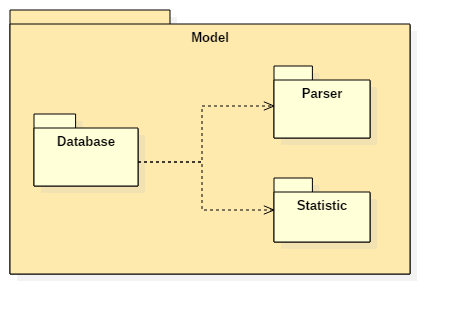
\includegraphics[scale=0.7]{../images/ModelPackage.png}
\end{center}
\end{figure}
\subsection{Model::Database}
\subsubsection{Model::Database::UserManager}
\begin{itemize}
\item\textbf{Funzione}:
\item\textbf{Relazioni con altre componenti}\\
La classe utilizza:
	\begin{itemize}
		\item
	\end{itemize}
\item\textbf{Attributi}:
	\begin{itemize}
		\item\code{}\\
		\item\code{}\\
		\item\code{}\\
		\item\code{}\\
	\end{itemize}
\item\textbf{Metodi}:
	\begin{itemize}
		\item\code{}\\
		\textbf{Parametri}:
			\begin{itemize}
				\item\code{}\\
			\end{itemize}
		\item\code{}\\
		\textbf{Parametri}:
			\begin{itemize}
				\item\code{}\\
			\end{itemize}
		\item\code{}\\
		\textbf{Parametri}:
			\begin{itemize}
				\item\code{}\\
			\end{itemize}
		\item\code{}\\
		\textbf{Parametri}:
			\begin{itemize}
				\item\code{}\\
			\end{itemize}
	\end{itemize}
\end{itemize}

\subsubsection{Model::Database::QuizManager}
\begin{itemize}
\item\textbf{Funzione}:
\item\textbf{Relazioni con altre componenti}\\
La classe utilizza:
	\begin{itemize}
		\item
	\end{itemize}
\item\textbf{Attributi}:
	\begin{itemize}
		\item\code{}\\
		\item\code{}\\
		\item\code{}\\
		\item\code{}\\
	\end{itemize}
\item\textbf{Metodi}:
	\begin{itemize}
		\item\code{}\\
		\textbf{Parametri}:
			\begin{itemize}
				\item\code{}\\
			\end{itemize}
		\item\code{}\\
		\textbf{Parametri}:
			\begin{itemize}
				\item\code{}\\
			\end{itemize}
		\item\code{}\\
		\textbf{Parametri}:
			\begin{itemize}
				\item\code{}\\
			\end{itemize}
		\item\code{}\\
		\textbf{Parametri}:
			\begin{itemize}
				\item\code{}\\
			\end{itemize}
	\end{itemize}
\end{itemize}

\subsubsection{Model::Database::QuestionManager}
\begin{itemize}
\item\textbf{Funzione}:
\item\textbf{Relazioni con altre componenti}\\
La classe utilizza:
	\begin{itemize}
		\item
	\end{itemize}
\item\textbf{Attributi}:
	\begin{itemize}
		\item\code{}\\
		\item\code{}\\
		\item\code{}\\
		\item\code{}\\
	\end{itemize}
\item\textbf{Metodi}:
	\begin{itemize}
		\item\code{}\\
		\textbf{Parametri}:
			\begin{itemize}
				\item\code{}\\
			\end{itemize}
		\item\code{}\\
		\textbf{Parametri}:
			\begin{itemize}
				\item\code{}\\
			\end{itemize}
		\item\code{}\\
		\textbf{Parametri}:
			\begin{itemize}
				\item\code{}\\
			\end{itemize}
		\item\code{}\\
		\textbf{Parametri}:
			\begin{itemize}
				\item\code{}\\
			\end{itemize}
	\end{itemize}
\end{itemize}

\subsection{Model::Parser}
\subsubsection{Model::Parser::Parser}
\begin{itemize}
\item\textbf{Funzione}:
\item\textbf{Relazioni con altre componenti}\\
La classe utilizza:
	\begin{itemize}
		\item
	\end{itemize}
\item\textbf{Attributi}:
	\begin{itemize}
		\item\code{}\\
		\item\code{}\\
		\item\code{}\\
		\item\code{}\\
	\end{itemize}
\item\textbf{Metodi}:
	\begin{itemize}
		\item\code{}\\
		\textbf{Parametri}:
			\begin{itemize}
				\item\code{}\\
			\end{itemize}
		\item\code{}\\
		\textbf{Parametri}:
			\begin{itemize}
				\item\code{}\\
			\end{itemize}
		\item\code{}\\
		\textbf{Parametri}:
			\begin{itemize}
				\item\code{}\\
			\end{itemize}
		\item\code{}\\
		\textbf{Parametri}:
			\begin{itemize}
				\item\code{}\\
			\end{itemize}
	\end{itemize}
\end{itemize}

\subsection{Model::Statistics}
\subsubsection{Model::Statistics::Statistics}
\begin{itemize}
\item\textbf{Funzione}:
\item\textbf{Relazioni con altre componenti}\\
La classe utilizza:
	\begin{itemize}
		\item
	\end{itemize}
\item\textbf{Attributi}:
	\begin{itemize}
		\item\code{}\\
		\item\code{}\\
		\item\code{}\\
		\item\code{}\\
	\end{itemize}
\item\textbf{Metodi}:
	\begin{itemize}
		\item\code{}\\
		\textbf{Parametri}:
			\begin{itemize}
				\item\code{}\\
			\end{itemize}
		\item\code{}\\
		\textbf{Parametri}:
			\begin{itemize}
				\item\code{}\\
			\end{itemize}
		\item\code{}\\
		\textbf{Parametri}:
			\begin{itemize}
				\item\code{}\\
			\end{itemize}
		\item\code{}\\
		\textbf{Parametri}:
			\begin{itemize}
				\item\code{}\\
			\end{itemize}
	\end{itemize}
\end{itemize}

\subsection{Model::Publishers}
\subsubsection{Model::Publishers::UserPublishers}
\begin{itemize}
\item\textbf{Funzione}:
\item\textbf{Relazioni con altre componenti}\\
La classe utilizza:
	\begin{itemize}
		\item
	\end{itemize}
\item\textbf{Attributi}:
	\begin{itemize}
		\item\code{}\\
		\item\code{}\\
		\item\code{}\\
		\item\code{}\\
	\end{itemize}
\item\textbf{Metodi}:
	\begin{itemize}
		\item\code{}\\
		\textbf{Parametri}:
			\begin{itemize}
				\item\code{}\\
			\end{itemize}
		\item\code{}\\
		\textbf{Parametri}:
			\begin{itemize}
				\item\code{}\\
			\end{itemize}
		\item\code{}\\
		\textbf{Parametri}:
			\begin{itemize}
				\item\code{}\\
			\end{itemize}
		\item\code{}\\
		\textbf{Parametri}:
			\begin{itemize}
				\item\code{}\\
			\end{itemize}
	\end{itemize}
\end{itemize}

\subsubsection{Model::Publishers::QuizPublishers}
\begin{itemize}
\item\textbf{Funzione}:
\item\textbf{Relazioni con altre componenti}\\
La classe utilizza:
	\begin{itemize}
		\item
	\end{itemize}
\item\textbf{Attributi}:
	\begin{itemize}
		\item\code{}\\
		\item\code{}\\
		\item\code{}\\
		\item\code{}\\
	\end{itemize}
\item\textbf{Metodi}:
	\begin{itemize}
		\item\code{}\\
		\textbf{Parametri}:
			\begin{itemize}
				\item\code{}\\
			\end{itemize}
		\item\code{}\\
		\textbf{Parametri}:
			\begin{itemize}
				\item\code{}\\
			\end{itemize}
		\item\code{}\\
		\textbf{Parametri}:
			\begin{itemize}
				\item\code{}\\
			\end{itemize}
		\item\code{}\\
		\textbf{Parametri}:
			\begin{itemize}
				\item\code{}\\
			\end{itemize}
	\end{itemize}
\end{itemize}

\subsubsection{Model::Publishers::QuestionPublishers}
\begin{itemize}
\item\textbf{Funzione}:
\item\textbf{Relazioni con altre componenti}\\
La classe utilizza:
	\begin{itemize}
		\item
	\end{itemize}
\item\textbf{Attributi}:
	\begin{itemize}
		\item\code{}\\
		\item\code{}\\
		\item\code{}\\
		\item\code{}\\
	\end{itemize}
\item\textbf{Metodi}:
	\begin{itemize}
		\item\code{}\\
		\textbf{Parametri}:
			\begin{itemize}
				\item\code{}\\
			\end{itemize}
		\item\code{}\\
		\textbf{Parametri}:
			\begin{itemize}
				\item\code{}\\
			\end{itemize}
		\item\code{}\\
		\textbf{Parametri}:
			\begin{itemize}
				\item\code{}\\
			\end{itemize}
		\item\code{}\\
		\textbf{Parametri}:
			\begin{itemize}
				\item\code{}\\
			\end{itemize}
	\end{itemize}
\end{itemize}
	\newpage
	\section{Package ViewModel}
\begin{figure}[h!]
\begin{center}
	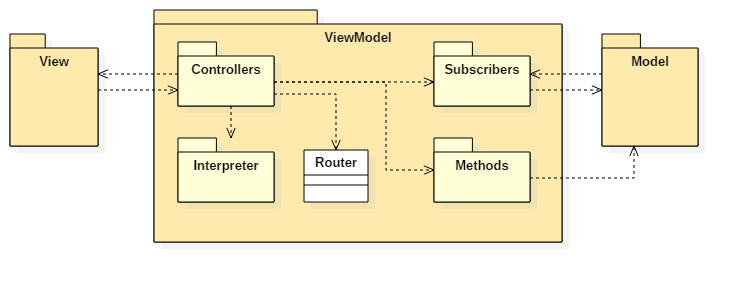
\includegraphics[scale=0.7]{../images/ViewModelPackage.png}
\end{center}
\end{figure}

\subsection{ViewModel::Subscribers}
\subsubsection{ViewModel::Subscribers::QuestionsSubscriber}
\begin{figure}[h!]
\begin{center}
	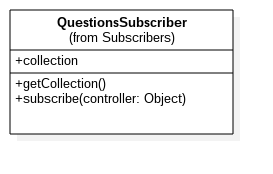
\includegraphics[scale=0.4]{../images/ViewModel/Subscribers/QuestionsSubscriber.png}
\end{center}
\end{figure}
\begin{itemize}
\item\textbf{Funzione del componente}: la classe è necessaria ad effettuare il \emph{subscribe} relativo alla collezione di domande del sistema;
	\item\textbf{Relazione d'uso con altre componenti}: \\
La classe utilizza:
	\begin{itemize}
		\item Model::Publishers::QuestionPublisher	
	\end{itemize}
\item\textbf{Attributi}:
	\begin{itemize}
		\item\code{- collection: String}: il nome della collezione sulla quale effettuare il subscribe.\\	
	\end{itemize}
\item\textbf{Metodi}:
	\begin{itemize}
		\item\code{+ getCollection(): String}: ritorna la collezione sulla quale può effettuare il subscribe.\\
		\textbf{Precondizioni}: viene richiesta la collezione di pertinenza della classe\\
		\textbf{Postcondizioni}: viene ritornato il nome della collezione\\
		\item\code{+ subscribe()}: metodo che effettua il subscribe del parametro controller alla collezione\\
		\textbf{Precondizioni}: viene richiesto di effettuare il subscribe del parametro controller alla collezione\\
		\textbf{Postcondizioni}: è stato effettuato il subscribe del controller alla collezione\\
		\textbf{Parametri}:
			\begin{itemize}
				\item\code{controller: Object}: il controller che necessita della collezione\\
			\end{itemize}
	\end{itemize}
\end{itemize}
\newpage

\subsubsection{ViewModel::Subscribers::QuizSubscriber}
\begin{figure}[h!]
\begin{center}
	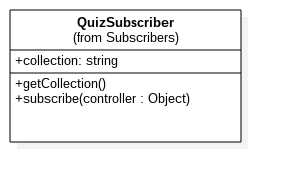
\includegraphics[scale=0.4]{../images/ViewModel/Subscribers/QuizSubscriber.png}
\end{center}
\end{figure}
\begin{itemize}
\item\textbf{Funzione del componente}: la classe è necessaria ad effettuare il \emph{subscribe} relativo alla collezione di quiz del sistema;
	\item\textbf{Relazione d'uso con altre componenti}:\\
La classe utilizza:
	\begin{itemize}
		\item Model::Publishers::QuizPublisher
	\end{itemize}
\item\textbf{Attributi}:
	\begin{itemize}
		\item\code{- collection: String}: il nome della collezione sulla quale effettuare il subscribe.\\	
	\end{itemize}
\item\textbf{Metodi}:
	\begin{itemize}
		\item\code{+ getCollection(): String}: ritorna la collezione sulla quale può effettuare il subscribe.\\
		\textbf{Precondizioni}: viene richiesta la collezione di pertinenza della classe\\
		\textbf{Postcondizioni}: viene ritornato il nome della collezione\\
		\item\code{+ subscribe()}: metodo che effettua il subscribe del parametro controller alla
		\textbf{Precondizioni}: viene richiesto di effettuare il subscribe del parametro controller alla collezione\\
		\textbf{Postcondizioni}: è stato effettuato il subscribe del controller alla collezione\\
		\textbf{Parametri}:
			\begin{itemize}
				\item\code{controller: Object}: il controller che necessita della collezione\\
			\end{itemize}
	\end{itemize}
\end{itemize}
\newpage

\subsection{ViewModel::Methods}
\subsubsection{ViewModel::Methods::QuestionMethods}
\begin{figure}[h!]
\begin{center}
	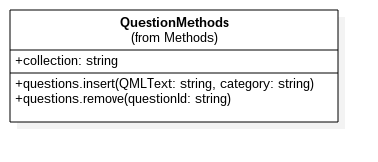
\includegraphics[scale=0.4]{../images/ViewModel/Methods/QuestionMethods.png}
\end{center}
\end{figure}
\begin{itemize}
\item\textbf{Funzione del componente}: permette al client di richiedere la modifica della collezione di domande del server;
	\item\textbf{Relazione d'uso con altre componenti}: \\
La classe utilizza:
	\begin{itemize}
		\item Model::Publishers::QuestionPublisher
		\item Model::Statistics::Statistics
	\end{itemize}
\item\textbf{Attributi}:
	\begin{itemize}
		\item\code{- collection: String}: la collezione sulla quale verranno implementati i methods\\
	\end{itemize}
\item\textbf{Metodi}:
	\begin{itemize}
		\item\code{+ questions.insert()}: metodo che inserisce una domanda nella collezione\\
		\textbf{Precondizioni}: viene richiesto di inserire una nuova domanda nella collezione\\
		\textbf{Postcondizioni}: la nuova domanda è stata salvata nel sistema\\
		\textbf{Parametri}:
			\begin{itemize}
				\item\code{QMLtext: string}: testo QML (corretto perchè viene prima parsato) corrispondente alla nuova domanda\\
				\item\code{category: string}: testo contente la categorie di appertenenza della domanda che si vuole inserire\\
			\end{itemize}
		\item\code{+ questions.remove()}: metodo che rimuove una domanda dalla collezione\\
		\textbf{Precondizioni}: viene richiesta l'eliminazione di una domanda dal sistema\\
		\textbf{Postcondizioni}: la domanda è stata eliminata dal sistema\\
		\textbf{Parametri}:
			\begin{itemize}
				\item\code{questionId: String}: identificativo univoco della domanda da rimuovere\\
			\end{itemize}
	\end{itemize}
\end{itemize}
\newpage

\subsubsection{ViewModel::Methods::QuizMethods}
\begin{figure}[h!]
\begin{center}
	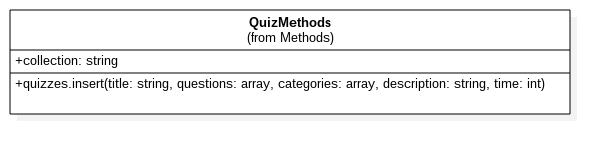
\includegraphics[scale=0.4]{../images/ViewModel/Methods/QuizMethods.png}
\end{center}
\end{figure}
\begin{itemize}
\item\textbf{Funzione del componente}: permette al client di richiedere la modifica della collezione di quiz del server;
	\item\textbf{Relazione d'uso con altre componenti}: \\
La classe utilizza:
	\begin{itemize}
		\item Model::Publishers::QuizPublisher
	\end{itemize}
\item\textbf{Attributi}:
	\begin{itemize}
		\item\code{- collection: String}: la collezione sulla quale verranno implementati i methods\\
	\end{itemize}
\item\textbf{Metodi}:
	\begin{itemize}
		\item\code{+ quizzes.insert()}: metodo che inserisce un quiz nella collezione\\
		\textbf{Precondizioni}: viene richiesto di inserire un nuovo quiz nella collezione\\
		\textbf{Postcondizioni}: il nuovo quiz è stato salvato nel sistema\\
		\textbf{Parametri}:
			\begin{itemize}
				\item\code{title: string}: contiene il titolo del nuovo questionario\\
				\item\code{questions: array}: elenca le domande presenti nel nuovo questionario\\
				\item\code{categories: array}: elenca le categorie di pertinenza del nuovo questionario\\
				\item\code{description: string}: contiene una breve descrizione testuale del questionario\\
				\item\code{time: int}: stabilisce il tempo massimo per la risoluzione del quiz\\
			\end{itemize}
		\item\code{+ quizzes.remove()}: metodo che rimuove un quiz dalla collezione\\
		\textbf{Precondizioni}: viene richiesta l'eliminazione di un quiz dal sistema\\
		\textbf{Postcondizioni}: il quiz è stato eliminato dal sistema\\
		\textbf{Parametri}:
			\begin{itemize}
				\item\code{quizId: String}: identificativo univoco della domanda da rimuovere\\
			\end{itemize}
	\end{itemize}
\end{itemize}
\newpage

\subsubsection{ViewModel::Methods::UserMethods}
\begin{figure}[h!]
\begin{center}
	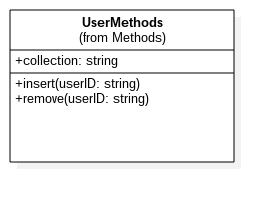
\includegraphics[scale=0.4]{../images/ViewModel/Methods/UserMethods.png}
\end{center}
\end{figure}
\begin{itemize}
\item\textbf{Funzione del componente}: permette al client di richiedere la modifica della collezione di utenti del server;
\item\textbf{Attributi}:
	\begin{itemize}
		\item\code{- collection: String}: la collezione sulla quale verranno implementati i methods\\
	\end{itemize}
\item\textbf{Metodi}:
	\begin{itemize}
		\item\code{+ insert()}: metodo che inserisce un utente nella collezione\\
		\textbf{Precondizioni}: viene richiesto di inserire un nuovo utente nella collezione\\
		\textbf{Postcondizioni}: il nuovo utente è stato salvato nel sistema\\
		\textbf{Parametri}:
			\begin{itemize}
				\item\code{userId: String}: identificativo univoco dell'utente da aggiungere\\
			\end{itemize}
		\item\code{+ remove()}: metodo che rimuove un utente dalla collezione\\
		\textbf{Precondizioni}: viene richiesta l'eliminazione di un utente dal sistema\\
		\textbf{Postcondizioni}: l'utente è stato eliminato dal sistema\\
		\textbf{Parametri}:
			\begin{itemize}
				\item\code{userId: String}: identificativo univoco dell'utente da rimuovere\\
			\end{itemize}
	\end{itemize}
\end{itemize}
\newpage

\subsection{ViewModel::Interpreter}
\subsubsection{ViewModel::Interpreter::Interpreter}
\begin{itemize}
\item\textbf{Funzione del componente}: interfaccia di base del tipo Interpreter.
	\item\textbf{Relazione d'uso con altre componenti}: viene concretizzata in\\ ViewModel::Interpreter::QMLInterpreter.\\
\end{itemize}
\subsubsection{ViewModel::Interpreter::InterpreterFactory}
\begin{figure}[h!]
\begin{center}
	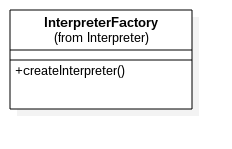
\includegraphics[scale=0.4]{../images/ViewModel/Interpreter/InterpreterFactory.png}
\end{center}
\end{figure}
\begin{itemize}
\item\textbf{Funzione del componente}: interfaccia di base delle Factory di tipi Interpreter.
	\item\textbf{Relazione d'uso con altre componenti}: viene concretizzata da\\ ViewModel::Interpreter::QMLInterpreterFactory.\\ 
\item\textbf{Attributi}: nessuno
\item\textbf{Metodi}:
	\begin{itemize}
		\item\code{+ createInterpreter(): Interpreter}: metodo astratto per la creazione di un Interpreter.\\
		\textbf{Precondizioni}: viene richiesta l'istanziazione di un Interpreter\\
		\textbf{Postcondizioni}: il nuovo Interpreter viene creato e ritornato al chiamante\\
	\end{itemize}
\end{itemize}

\subsubsection{ViewModel::Interpreter::QMLInterpreterFactory}
\begin{figure}[h!]
\begin{center}
	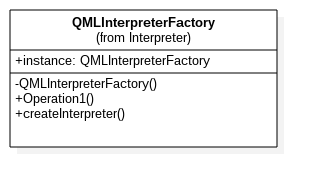
\includegraphics[scale=0.4]{../images/ViewModel/Interpreter/QMLInterpreterFactory.png}
\end{center}
\end{figure}
\begin{itemize}
\item\textbf{Funzione del componente}: crea oggetti di tipo QMLInterpreter.
	\item\textbf{Relazione d'uso con altre componenti}: è concretizzazione dalla classe\\ ViewModel::Interpreter::InterpreterFactory. Crea oggetti QMLInterpreter.\\
\item\textbf{Attributi}:
	\begin{itemize}
		\item\code{- instance: QMLInterpreterFactory}: campo dati statico che rappresenta l'unica istanza della classe\\
	\end{itemize}
\item\textbf{Metodi}:
	\begin{itemize}
		\item\code{- QMLInterpreterFactory()}: costruttore privato della classe\\
		\item\code{+ getInstance(): QMLInterpreterFactory}: metodo che ritorna l'unica istanza della classe\\
		\textbf{Precondizioni}: viene richiesta la factory QMLInterpreterFactory\\
		\textbf{Postcondizioni}: l'unica istanza della factory viene ritornata al chiamante. Se la factory non esisteva è stata creata.\\
		\item\code{+ createInterpreter(): QMLInterpreter}: metodo ereditato da InterpreterFactorye concretizzato per la creazione di un interprete di tipo QMLInterpreter.\\
		\textbf{Precondizioni}: viene richiesta l'istanziazione di un QMLInterpreter\\
		\textbf{Postcondizioni}: il nuovo QMLInterpreter viene creato e ritornato al chiamante\\
	\end{itemize}
\end{itemize}

\subsubsection{ViewModel::Interpreter::QMLInterpreter}
\begin{figure}[h!]
\begin{center}
	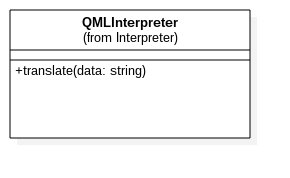
\includegraphics[scale=0.4]{../images/ViewModel/Interpreter/QMLInterpreter.png}
\end{center}
\end{figure}
\begin{itemize}
\item\textbf{Funzione del componente}: classe astratta che rappresenta gli Interpreter che traducono codice QML in un altro formato.
	\item\textbf{Relazione d'uso con altre componenti}: è sottotipo di ViewModel::Interpreter::Interpreter. Viene concretizzata in ViewModel::Interpreter::QML2HTMLInterpreter.\\ 
\item\textbf{Attributi}: Nessuno
\item\textbf{Metodi}:
	\begin{itemize}
		\item\code{translate(): String}: metodo astratto ereditato da Interpreter\\\\
		\textbf{Precondizioni}: viene richiesta la traduzione di un testo QML\\
		\textbf{Postcondizioni}: il testo QML è stato tradotto in un altro linguaggio\\
		\textbf{Parametri}:
			\begin{itemize}
				\item\code{data: String}: l'input QML che deve essere tradotto \\
			\end{itemize}
	\end{itemize}
\end{itemize}

\subsubsection{ViewModel::Interpreter::QML2HTMLInterpreter}
\begin{figure}[h!]
\begin{center}
	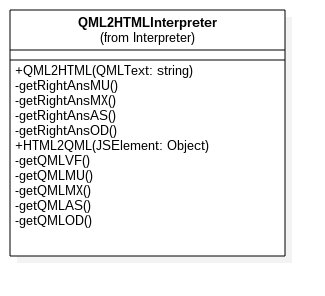
\includegraphics[scale=0.4]{../images/ViewModel/Interpreter/QML2HTMLInterpreter.png}
\end{center}
\end{figure}
\begin{itemize}
	\item\textbf{Funzione del componente}: traduce codice QML in codice HTML.
	\item\textbf{Relazione d'uso con altre componenti}: la classe è concretizzazione di\\ ViewModel::Interpreter::QMLInterpreter.\\
	\item\textbf{Metodi}:
	\begin{itemize}
		\item\code{+ QML2HTML(): String}:\\
		 metodo per la traduzione da QML ad HTML. Questo metodo prende in input un file di testo in formato QML restituisce un elemento JavaScript da utilizzare nella pagina HTML per la visualizzazione della domanda \\
		\textbf{Parametri}:
			\begin{itemize}
				\item\code{QMLText: String}:\\
				 l'input testuale che deve essere convertito \\
			\end{itemize}
		\textbf{Precondizioni}: viene richiesta la conversione di un testo QML in un elemento Javascript\\
		\textbf{Postcondizioni}: il testo è stato convertito ed è stato restituito un elemento javascript definito\\
		\item\code{- getRightAnsMU(): Object}\\
		 \\Metodo che restituisce la risposta giusta per il tipo MU\\
		\textbf{Precondizioni}: la funzione QML2HTML() ha preso in input il testo in formato QML ed è stata creata e definita la variabile m di tipo array che contiene i risultati della funzione exec() chiamata in QML2HTML()\\
		\textbf{Postcondizioni}: viene restituita l'unica risposta corretta \\
		
		\item\code{- getRightAnsMX(): Object}\\
		 \\Metodo che restituisce la risposta giusta per il tipo MX\\
		\textbf{Precondizioni}: la funzione QML2HTML() ha preso in input il testo in formato QML ed è stata creata e definita la variabile m di tipo array che contiene i risultati della funzione exec() chiamata in QML2HTML()\\
		\textbf{Postcondizioni}: vengono restituite le risposte corrette \\
		
		\item\code{- getRightAnsAS(): Object}\\
		 \\Metodo che restituisce la risposta giusta per il tipo AS\\
		\textbf{Precondizioni}: la funzione QML2HTML() ha preso in input il testo in formato QML ed è stata creata e definita la variabile m di tipo array che contiene i risultati della funzione exec() chiamata in QML2HTML()\\
		\textbf{Postcondizioni}: vengono restituiti due array di elementi che rappresentano l'insieme A e l'insieme B. Ogni elemento di un insieme è composto dal testo della risposta e dal suo numero identificativo \\
		
		\item\code{- getRightAnsOD(): Object}\\
		 \\Metodo che restituisce la risposta giusta per il tipo OD\\
		\textbf{Precondizioni}: la funzione QML2HTML() ha preso in input il testo in formato QML ed è stata creata e definita la variabile m di tipo array che contiene i risultati della funzione exec() chiamata in QML2HTML()\\
		\textbf{Postcondizioni}: viene restituito un array di elementi in cui ogni elemento è composto dal testo della risposta e dal suo identificativo di posizio \\
		
		\item\code{+ HTML2QML(): String}:\\
		 metodo per la conversione di un elemento domanda da JSObject a QML. Questo metodo prende in input un elemento JavaScript prodotto dal form di creazione domanda e restituisce una stringa in formato QML. \\
		\textbf{Parametri}:
			\begin{itemize}
				\item\code{JSObject}: Object\\
				 L'oggetto JavaScript da convertire in QML \\
			\end{itemize}
		\textbf{Precondizioni}: viene richiesta la conversione di un elemento Javascrip in un testo QML, l'elemento deve essere stato quindi definito\\
		\textbf{Postcondizioni}: viene restituita una variabile stringa in formato QML\\
		\item\code{- getQMLVF(): string}\\
		 Metodo che restituisce la stringa QML dell'elemento domanda di tipo Vero/Falso\\
		\textbf{Precondizioni}: la funzione HTML2QML() ha preso in input l'elemento JavaScript per la conversione\\
		\textbf{Postcondizioni}: viene restituita una variabile stringa in formato QML\\
		
		\item\code{- getQMLMU(): string}\\
		 Metodo che restituisce la stringa QML dell'elemento domanda di tipo risposta multipla\\
		\textbf{Precondizioni}: la funzione HTML2QML() ha preso in input l'elemento JavaScript per la conversione\\
		\textbf{Postcondizioni}: viene restituita una variabile stringa in formato QML \\
		
		\item\code{- getQMLMX(): string}\\
		 Metodo che restituisce la stringa QML dell'elemento domanda di tipo risposta multipla a più risposte giuste possibili\\
		\textbf{Precondizioni}: la funzione HTML2QML() ha preso in input l'elemento JavaScript per la conversione\\
		\textbf{Postcondizioni}: viene restituita una variabile stringa in formato QML \\
		
		\item\code{- getQMLAS(): string}\\
		 Metodo che restituisce la stringa QML dell'elemento domanda di tipo associazione\\
		\textbf{Precondizioni}: la funzione HTML2QML() ha preso in input l'elemento JavaScript per la conversione\\
		\textbf{Postcondizioni}: viene restituita una variabile stringa in formato QML \\
		
		\item\code{- getQMLOD(): string}\\
		 Metodo che restituisce la stringa QML dell'elemento domanda di tipo ordinamento\\
		\textbf{Precondizioni}: la funzione HTML2QML() ha preso in input l'elemento JavaScript per la conversione\\
		\textbf{Postcondizioni}: viene restituita una variabile stringa in formato QML \\
		
	\end{itemize}
\end{itemize}
\newpage

\subsection{ViewModel::Router}
\subsubsection{ViewModel::Router::Router}
\begin{figure}[h!]
\begin{center}
	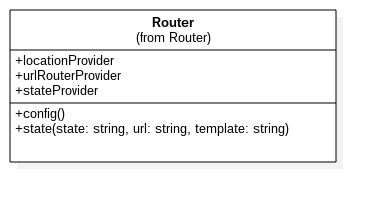
\includegraphics[scale=0.4]{../images/ViewModel/Router/Router.png}
\end{center}
\end{figure}
\begin{itemize}
\item\textbf{Funzione del componente}: implementa il routing dinamico dell'applicazione. Permette di dividere la parte statica dell'applicazione dalla parte che viene elaborata dinamicamente;
\item\textbf{Attributi}:
	\begin{itemize}
		\item\code{\$locationProvider: \$locationProvider}: provider AngularJs per rendere gli Url più leggibili\\
		\item\code{\$urlRouterProvider: \$urlRouterProvider}: modulo del package ui-router per definire il routing di default dell'applicazione\\
		\item\code{\$stateProvider: \$stateProvider}: modulo del package ui-router per mappare gli Url al caricamento dinamico dei template dell'applicazione. Tale associazione è definita come uno 'state'\\
	\end{itemize}
\item\textbf{Metodi}:
	\begin{itemize}
		\item\code{config()}: si occupa di gestire le varie chiamate del metodo state() all'inizializzazione dell'applicazione\\
		\textbf{Precondizioni}: l'applicazione Quizzipedia viene avviata\\
		\textbf{Postcondizioni}: tutti i template sono disponibili al caricamento\\
		\item\code{state()}: metodo per collegare un Url dell'applicazione al rispettivo template da caricare\\
		\textbf{Precondizioni}: viene richiesta l'associazione di un Url al caricamento di un template\\
		\textbf{Postcondizioni}: un Url univoco è stato associato al caricamento dinamico di uno specifico template\\
		\textbf{Parametri}:
			\begin{itemize}
				\item\code{state: String}: il nome dello stato rappresentato dall'associazione Url-Template\\
				\item\code{url: String}: l'Url sul quale effettuare il matching\\
				\item\code{template: String}: il template da caricare una volta trovato il match\\
			\end{itemize}
	\end{itemize}
\end{itemize}
\newpage

\subsection{ViewModel::Controller}
\subsubsection{ViewModel::Controller::QuestionList}
\begin{figure}[h!]
\begin{center}
	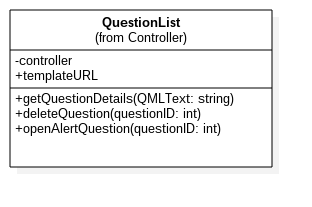
\includegraphics[scale=0.6]{../images/ViewModel/Controller/QuestionList.png}
\end{center}
\end{figure}
\begin{itemize}
\item\textbf{Funzione del componente:} visualizza una lista di domande
				\item\textbf{Relazioni d'uso con altre componenti:} \\
La classe si relaziona con:
	\begin{itemize}
		\item View::Templates::Question
		\item View::Templates::QuestionList
		\item Model::Publishers::QuestionPublishers
		\item ViewModel::Interpreter::Interpreter	
	\end{itemize}
\item\textbf{Funzionalità}:
\begin{itemize}
		\item\code{+ getQuestionDetails(QMLtext)}: restituisce i dettagli sulla domanda corrente se essa è valida;\\
		\item\code{+ deleteQuestion(questionID)}: richiede la rimozione dal database di una domanda;\\
		\item\code{+ openAlertQuestion(questionID)}: fornisce un messaggio pop-up di conferma all'utente;\\
	\end{itemize}
	\item\textbf{Attributi:}
	\begin{itemize}
	\item\code{+ controller: String}: variabile contenente il nome del controller del template;\\
 
 	\item\code{+ templateUrl: String}: stringa contenente il percorso del file HTML che contiene il template\\
	\end{itemize}
\end{itemize}
\newpage

\subsubsection{ViewModel::Controller::Question}
\begin{figure}[h!]
\begin{center}
	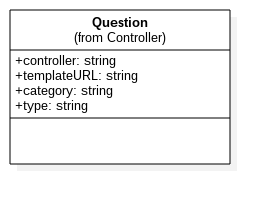
\includegraphics[scale=0.6]{../images/ViewModel/Controller/Question.png}
\end{center}
\end{figure}
\begin{itemize}
\item\textbf{Funzione del componente:} permette la visualizzazione di una singola domanda
				\item\textbf{Relazioni d'uso con altre componenti:} 
La classe è in relazione con:
\begin{itemize}
		\item View::Templates::Question
		\item View::Templates::QuestionList
	\end{itemize}
\item\textbf{Attributi}:
	\begin{itemize}
		\item\code{+ controller: String}: variabile contenente il nome del controller del template;\\

		\item\code{+ templateUrl: String}: stringa contenente il percorso del file HTML che contiene il template\\
		\item\code{+ category: String}: stringa contenente la categoria della domanda
 		\item\code{+ type: String}: stringa contenente il tipo della domanda
	\end{itemize}
\end{itemize}
\newpage

\subsubsection{ViewModel::Controller::QuizList}
\begin{figure}[h!]
\begin{center}
	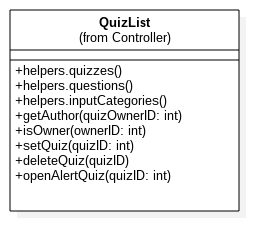
\includegraphics[scale=0.6]{../images/ViewModel/Controller/QuizList.png}
\end{center}
\end{figure}
\begin{itemize}
\item\textbf{Funzione del componente:} permette visualizzazione e interazione di una lista di questionari
				\item\textbf{Relazioni d'uso con altre componenti:}\\
La classe utilizza:
	\begin{itemize}
		\item View::Templates::Quiz
		\item Model::Publishers::QuizPublishers
		\item Model::Publishers::QuestionPublishers
		\item Model::Parser::Parser
	\end{itemize}
\item\textbf{Funzionalità}:
	\begin{itemize}
		\item\code{+ helpers.quizzes()}: restituisce i questionari della categoria ricercata;\\
		\item\code{+ helpers.questions()}: restituisce le domande contenute nel questionario selezionato;\\
		\item\code{+ helpers.inputCategories()}: recupera tutte le categorie dei quiz per popolare la select senza inserire duplicati;\\
		\item\code{+ getAuthor(quizOwnerID)}: restituisce l'autore del quiz selezionato\\
		\item\code{+ isOwner(ownerID)}: restituisce un esito positivo se il creatore del quiz è l'utente attualmente loggato\\
		\item\code{+ setQuiz(qID}: richiede il questionario scelto dall'utente per il caricamento dal database\\
		\item\code{+ deleteQuiz(quiz)}: permette l'eliminazione del quiz scelto\\
		\item\code{+ openAlertQuiz(quizID)}: fornisce un messaggio pop-up di conferma all'utente;\\
	\end{itemize}
\end{itemize}
\newpage

\subsubsection{ViewModel::Controller::Quiz}
\begin{figure}[h!]
\begin{center}
	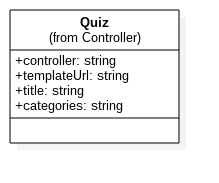
\includegraphics[scale=0.6]{../images/ViewModel/Controller/Quiz.png}
\end{center}
\end{figure}
\begin{itemize}
\item\textbf{Funzione del componente:} visualizza un quiz inserito in una lista
				\item\textbf{Relazioni d'uso con altre componenti:}\\
 La classe è utilizzata da:
 	\begin{itemize}
 		\item View::Templates::QuizList
 		\item View::Templates::Quiz
 		\item View::Templates::QuestionList
 	\end{itemize}
 \item\textbf{Attributi}:
 	\begin{itemize}
 		\item\code{+ controller: String}: variabile contenente il nome del controller del template;\\
		
		\item\code{+ templateUrl: String}: stringa contenente il percorso del file HTML che contiene il template\\
		\item\code{title: String}: stringa contenente il titolo del quiz
		\item\code{categories: String}: stringa contenente le categorie del quiz
 	\end{itemize}
 \end{itemize}
\newpage

 \subsubsection{ViewModel::Controller::QuestionForm}
 \begin{figure}[h!]
\begin{center}
	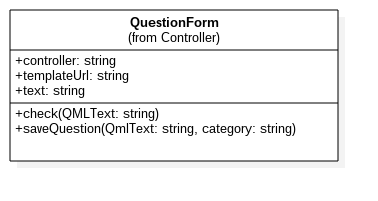
\includegraphics[scale=0.6]{../images/ViewModel/Controller/QuestionForm.png}
\end{center}
\end{figure}
 \begin{itemize}
 \item\textbf{Funzione del componente:} visualizza il form utilizzabile sia per la creazione che per la modifica di una domanda
 \item\textbf{Attributi}:
 	\begin{itemize}
 		\item\code{+ controller: String}: variabile contenente il nome del controller del template;\\
		
		\item\code{+ templateUrl: String}: stringa contenente il percorso del file HTML che contiene il template\\
		\item\code{+ category: String}: stringa contenente la categoria della domanda
		\item\code{+ text: String}: stringa contenente il testo della domanda
 	\end{itemize}
 	\item\textbf{Metodi}:
 	\begin{itemize}
 		\item\code{+ check(QMLtext)}: si occupa della verifica della correttezza del testo QML inserito dall'utente;\\
 		\item\code{+ saveQuestion(QMLtext, category)}: salva le modifiche effettuate su una domanda;\\
 	\end{itemize}
 \end{itemize}
\newpage
 
 \subsubsection{ViewModel::Controller::QuizCreationForm}
 \begin{figure}[h!]
\begin{center}
	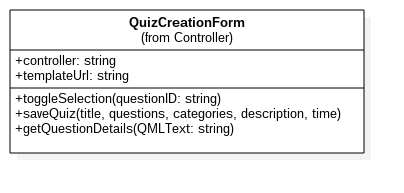
\includegraphics[scale=0.6]{../images/ViewModel/Controller/QuizCreationForm.png}
\end{center}
\end{figure}
 \begin{itemize}
 \item\textbf{Funzione del componente:} visualizza il form di creazione di un questionario
 \item\textbf{Relazione d'uso con altri componenti}:
 \begin{itemize}
 	\item View::Pages::QuizCreationPage
 	\item Model::Publishers::QuestionPublishers
 \end{itemize}
 \item\textbf{Attributi}:
 	\begin{itemize}
 		\item\code{+ controller: String}: variabile contenente il nome del controller del template;\\
		
		\item\code{+ templateUrl: String}: stringa contenente il percorso del file HTML che contiene il template\\
 	\end{itemize}
 	\item\textbf{Metodi};
 	\begin{itemize}
 		\item\code{+ toggleSelection(questionID)}: si occupa di gestire la selezione della domanda da inserire nel questionario attualmente in fase di creazione;\\
 		\item\code{+ savequiz(title,questions,categories,description,time)}:
 		gestisce il salvataggio del questionario;\\
 		\item\code{+ getQuestionDetails(QMLtext)}: fornisce informazioni su una specifica domanda candidata all'inserimento nel questionario;\\
 	\end{itemize}
 \end{itemize}
\newpage
 
 \subsubsection{ViewModel::Controller::QuestionCompilation}
 \begin{figure}[h!]
\begin{center}
	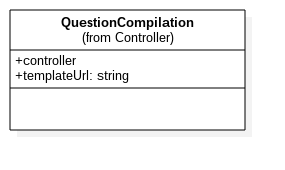
\includegraphics[scale=0.6]{../images/ViewModel/Controller/QuestionCompilation.png}
\end{center}
\end{figure}
 \begin{itemize}
 \item\textbf{Funzione del componente:} visualizza una domanda e ne permette la compilazione
 \item\textbf{Relazioni con altre componenti}\\
 La classe utilizza:
 	\begin{itemize}
 		\item View::Templates::Question
 		\item View::Templates::QuizResults
 	\end{itemize}
 \item\textbf{Attributi}:
 	\begin{itemize}
 		\item\code{+ controller: String}: variabile contenente il nome del controller del template;\\
		
		\item\code{+ templateUrl: String}: stringa contenente il percorso del file HTML che contiene il template\\
 	\end{itemize}
 \end{itemize}
\newpage
 
 \subsubsection{ViewModel::Controller::QuizResults}
 \begin{figure}[h!]
\begin{center}
	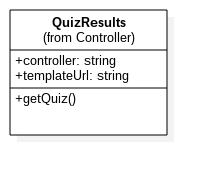
\includegraphics[scale=0.6]{../images/ViewModel/Controller/QuizResults.png}
\end{center}
\end{figure}
 \begin{itemize}
 \item\textbf{Funzione del componente:} visualizza i risultati ottenuti in seguito alla compilazione di un quiz
 \item\textbf{Relazioni con altre componenti}\\
 La classe utilizza:
 	\begin{itemize}
 		\item View::Templates::QuestionCompilation
 		\item View::Templates::QuizResults
 	\end{itemize}
 \item\textbf{Attributi}:
 	\begin{itemize}
 		\item\code{+ controller: String}: variabile contenente il nome del controller del template;\\
		\item\code{+ templateUrl: String}: stringa contenente il percorso del file HTML che contiene il template\\
 	\end{itemize}
 	\item\textbf{Metodi}:
 	\begin{itemize}
 		\item\code{+ getQuiz()}: si occupa di fornire il punteggio finale
 	\end{itemize}
 \end{itemize}
\newpage
 
 \subsubsection{ViewModel::Controller::SearchForm}
 \begin{figure}[h!]
\begin{center}
	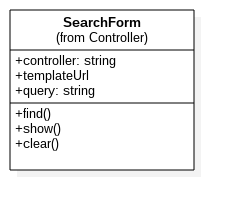
\includegraphics[scale=0.6]{../images/ViewModel/Controller/SearchForm.png}
\end{center}
\end{figure}
 \begin{itemize}
 \item\textbf{Funzione del componente:} visualizza una form per l’inserimento dei dati desiderati e l’avvio della ricerca
 \item\textbf{Attributi}:
 	\begin{itemize}
 		\item\code{+ controller: String}: variabile contenente il nome del controller del template;\\
		
		\item\code{+ templateUrl: String}: stringa contenente il percorso del file HTML che contiene il template\\
		\item\code{+ query: String}: stringa contenente la query da sottomettere al sistema\\
 	\end{itemize}
 	\item\textbf{Funzionalità}:
 	\begin{itemize}
 		\item\code{+ find():} esegue l'effettiva attività di ricerca nel sistema\\
		\item\code{+ show():} fornisce la rappresentazione grafica dei risultati\\
		\item\code{+ clear():} metodo di servizio per la pulizia dell'interfaccia\\
 	\end{itemize}
 \end{itemize}
\newpage
 
 \subsubsection{ViewModel::Controller::NavBar}
 \begin{figure}[h!]
\begin{center}
	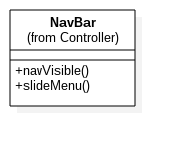
\includegraphics[scale=0.6]{../images/ViewModel/Controller/NavBar.png}
\end{center}
\end{figure}
 \begin{itemize}
 \item\textbf{Funzione del componente:} Fornisce un menù laterale che facilita l'interazione dell'utente con l'applicazione
 \item\textbf{Relazione con altri componenti:}
 \begin{itemize}
 	\item View::Templates::navbar
 \end{itemize}
 \item\textbf{Funzionalità}:
 	\begin{itemize}
 		\item\code{+ navVisible():} imposta la larghezza del menù laterale\\
		\item\code{+ slideMenu():} gestisce effetti grafici responsive\\
 	\end{itemize}
 \end{itemize}
\newpage
 
 \subsubsection{ViewModel::Controller::TopBar}
 \begin{itemize}
 \item\textbf{Funzione del componente:} Fornisce il menù orizzontale con cui l'utente può interfacciarsi con il sistema
 \item\textbf{Relazione con altri componenti:}
 \begin{itemize}
 	\item View::Templates::topbar
 \end{itemize}
 \end{itemize}
\newpage
 
  \subsubsection{ViewModel::Controller::UserProfile}
  \begin{figure}[h!]
\begin{center}
	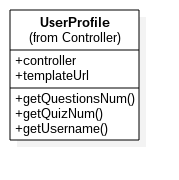
\includegraphics[scale=0.6]{../images/ViewModel/Controller/UserProfile.png}
\end{center}
\end{figure}
 \begin{itemize}
 \item\textbf{Funzione del componente:} permette la visualizzazione e l'interazione dell'utente con il proprio profilo e le funzionalità da esso offerto\\
 \item\textbf{Relazione con altri componenti:}
 \begin{itemize}
 	\item View::Templates::UserProfile
 	\item ViewModel::Controller::QuestionList
 	\item ViewModel::Controller::QuizList
 	\item Model::Publishers::QuestionPublishers
 	\item Model::Publishers::QuizPublishers
 \end{itemize}
 \item\textbf{Attributi:}
 \begin{itemize}
 	\item\code{+ controller: String}: variabile contenente il nome del controller del template;\\
		\item\code{+ templateUrl: String}: stringa contenente il percorso del file HTML che contiene il template\\
 \end{itemize}
 \item\textbf{Metodi:}
 	\begin{itemize}
 		\item\code{+ getQuestionsNum():} ritorna la quantità di domande create dallo stesso utente;\\
		\item\code{+ getQuizNum():} ritorna la quantità di questionari creati dallo stesso utente;\\
		\item\code{+ getUsername():} ritorna il nome dell'utente loggato;\\
 	\end{itemize}
 \end{itemize}
\newpage
 
 \subsubsection{ViewModel::Controller::QuizHome}
 \begin{itemize}
 \item\textbf{Funzione del componente:} istanzia il template per la visualizzazione della pagina principale
 \item\textbf{Relazione con altri componenti:}
 \begin{itemize} 
	\item View::Templates::QuizHome
	\item View::Quizzipedia
 \end{itemize}
 \end{itemize}
\newpage

 \subsubsection{ViewModel::Controller::QuizStatistics}
  \begin{itemize}
 \item\textbf{Funzione del componente:} istanzia il template per la visualizzazione delle statistiche dettagliate per una determinata domanda o questionario
 \item\textbf{Relazione con altri componenti:}
 \begin{itemize}
		\item View::Templates::QuizStatistics
		\item View::Templates::QuizResults
 \end{itemize}
 \end{itemize}
\newpage

 \subsubsection{ViewModel::Controller::QuizCompilation}
 \begin{figure}[h!]
\begin{center}
	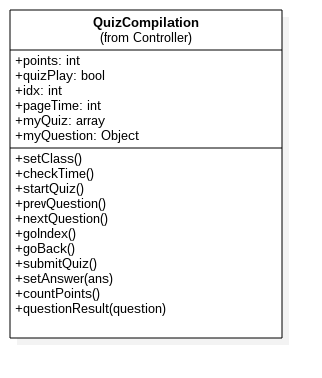
\includegraphics[scale=0.6]{../images/ViewModel/Controller/QuizCompilation.png}
\end{center}
\end{figure}
  \begin{itemize}
 \item\textbf{Funzione del componente:} gestisce l'intera compilazione di un questionario
 \item\textbf{Relazione con altri componenti:}
 \begin{itemize}
	\item View::Templates::QuizCompilation
	\item ViewModel::Interpreter::Interpreter
 \end{itemize}
 \item\textbf{Attributi:}
 \begin{itemize}
		\item\code{punti: int} mantiene il punteggio corrente dell'utente
		\item\code{quizPlay: bool} vera se il questionario è in esecuzione, falsa altrimenti
		\item\code{idx: int} indice della domanda correntemente visualizzata
		\item\code{pageTime: int} contatore contenente il tempo rimanente
		\item\code{myQuiz: array} array che contiene il questionario caricato
		\item\code{myQuestion: object} contiene la singola domanda attualmente visualizzata
 \end{itemize}
 \item\textbf{Metodi:}
 	\begin{itemize}
\item setClass()
\begin{itemize}
	\item{Precondizione: L'utente seleziona una domanda}
	\item{Postcondizione: La domanda su cui è stato invocato il metodo viene visualizzata}
\end{itemize}
\item checkTime()
\begin{itemize}
	\item{Precondizione: Viene richiesto il tempo rimanente}
	\item{Postcondizione: Viene restituito il tempo rimanente ed eventualmente viene forzata la consegna}
\end{itemize}
\item startQuiz()
\begin{itemize}
	\item{Precondizione: L'utente ha richiesto un questionario per lo svolgimento}
	\item{Postcondizione: Il questionario prescelto è in esecuzione}
\end{itemize}
\item prevQuestion()
\begin{itemize}
	\item{Precondizione: L'utente ha cliccato sul tasto Domanda Precedente}
	\item{Postcondizione: Viene visualizzata la domanda precedente}
\end{itemize}
\item nextQuestion()
\begin{itemize}
	\item{Precondizione: L'utente ha cliccato sul tasto Domanda Successiva}
	\item{Postcondizione: Viene visualizzata la domanda successiva}
\end{itemize}
\item goIndex(index)
\begin{itemize}
	\item{Precondizione: L'utente seleziona una domanda nella barra delle domande}
	\item{Postcondizione: La domanda selezionata viene visualizzata}
\end{itemize}
\item goBack()
\begin{itemize}
	\item{Precondizione: L'utente clicca sul tasto Esci}
	\item{Postcondizione: Il questionario viene terminato e non consegnato, viene visualizzata la pagina di selezione del questionario}
\end{itemize}
\item submitQuiz()
\begin{itemize}
	\item{Precondizione: L'utente clicca sul tasto Consegna}
	\item{Postcondizione: Viene consegnato il quiz che verrà poi valutato dal sistema}
\end{itemize}
\item setAnswer(ans)
\begin{itemize}
	\item{Precondizione: L'utente ha selezionato una risposta}
	\item{Postcondizione: La risposta viene registrata come data}
\end{itemize}
\item countPoints()
\begin{itemize}
	\item{Precondizione: viene richiesto il conteggio totale dei punti effettuati}
	\item{Postcondizione: viene restituito il punteggio corrente}
\end{itemize}
\item questionResult(question)
\begin{itemize}
	\item{Precondizione: viene richiesta la verifica della correttezza di una risposta data dall'utente}
	\item{Postcondizione: viene attribuito un punteggio positivo in caso di riposta corretta}
\end{itemize}
 	\end{itemize}
 \end{itemize}
	\newpage
	\section{Tracciamento}
\subsection{Mappatura classi - requisiti}
\begin{longtable}{p{0.8\textwidth}p{0.20\textwidth}}

\caption{Mappatura delle classi sui requisiti} \\

Nome classe & Codice requisito \\
\midrule
\endfirsthead

Nome classe & Codice requisito \\
\midrule
\endhead

\multicolumn{2}{c}{\footnotesize\itshape\tablename~\thetable: Mappatura delle classi sui requisiti}
\endfoot

\multicolumn{2}{c}{\footnotesize\itshape\tablename~\thetable: Mappatura delle classi sui requisiti}
\endlastfoot
	
%  M	O	D	E	L

Model::Database 			& F 1.2.2\\
							& F 3\\
							& F 3.1.1\\
							& F 3.2\\
							& F 6.2.2\\
\midrule
Model::Database::QuestionManager::AddQuestion	& F 5\\
												& F 5.1\\
												& F 5.2\\

\midrule
Model::Database::QuestionManager::ModifyQuestion	& F 5.3\\
									
\midrule
Model::Database::QuestionManager::RemoveQuestion	& F 5.4\\

\midrule
Model::Database::QuizManager::AddQuiz	& F 6\\
										& F 6.1\\
										& F 6.2\\

\midrule
Model::Database::QuizManager::RemoveQuiz	& Non tracciabile\\

\midrule
Model::Database::UserManager::LogIn	& F 2\\
									& F 2.2\\
\midrule
Model::Database::UserManager::AddUser	& F 1\\
										& F 2.3.2\\
										
\midrule
Model::Database::UserManager::RemoveUser	& Non tracciabile\\

\midrule
Model::Parser::Parser		& F 5.2.1\\
							& F 8\\

\midrule
Model::Statistics::Statistics	& 4.5.2\\
								& 4.5.2.1\\
								& 4.5.2.1.1\\
								& 4.5.2.1.2\\
								& 4.5.2.1.3\\

\midrule
Model::Publishers::UserPublishers	& Non tracciabile\\

\midrule
Model::Publishers::QuizPublishers	& Non tracciabile\\

\midrule
Model::Publishers::QuestionPublishers	& Non tracciabile\\

%  V	I	E	W 

\midrule
View::Pages::RegistrationPage	& F 1\\
								& F 1.1\\
								& F 1.1.1\\
								& F 1.1.2\\
								& F 1.1.2.1\\
								& F 1.2\\
								& F 1.2.1.1\\
								& F 1.2.1.2\\
								& F 1.2.3\\
\midrule
View::Pages::LoginPage			& F 2\\
								& F 2.1\\
								& F 2.1.1\\
								& F 2.1.2\\
								& F 2.3\\
								& F 2.3.1\\
								& F 2.3.1.1\\
								& F 2.3.2\\
								
\midrule
View::Pages::CategoryListPage					& F 3.1\\
								& F 3.1.1\\
								& F 3.1.2\\
								& F 3.1.3\\

\midrule
View::Pages::QuizListPage					& F 3\\
								& F 3.1\\
								& F 3.1.1\\
								& F 3.1.2\\
								& F 3.1.3\\
								& F 3.2\\
								& F 3.2.1\\
								& F 3.2.2\\
								& F 3.2.3\\
								
\midrule
View::Pages::QuizExecutionPage	& F 4\\
								& F 4.1\\
								& F 4.2.1\\
								& F 4.2.2\\
								& F 4.2.3\\
								& F 4.2.4\\
								& F 4.2.4.1\\
								& F 4.2.5\\
								& F 4.2.5.1\\
								& F 4.2.6\\
								& F 4.2.6.1\\
								& F 4.2\\
								& F 4.3\\
								& F 4.4\\
								& F 4.5\\
								& F 4.5.1\\
								& F 4.5.2.1\\
								& F 4.5.2.1\\
								& F 4.5.2.1.1\\
								& F 4.5.2.1.2\\
								& F 4.5.2.1.3\\
								& F 4.6.2\\
& F 4.7\\

\midrule
View::Pages::PasswordRecoveryPage	& F 2.2\\
								& F 2.2.1\\
								& F 2.2.2\\
								& F 2.2.2.1\\
								& F 2.2.2.2\\
								& F 2.2.3\\

\midrule
View::Pages::QuizResultPage	& 4.5.2\\
								& 4.5.2.1\\
								& 4.5.2.1.1\\
								& 4.5.2.1.2\\
								& 4.5.2.1.3\\	
							
\midrule
View::Pages::QuizManagementPage	& F 6\\

\midrule
View::Pages::ViewTutorialPage	& F 8.3\\

\midrule
View::Pages::QuizCreationPage	& F 6\\

\midrule
View::Pages::QuestionCreationPage	& F 5\\

\midrule
View::Pages::QuestionUpdatePage	& F 5.3\\

% templates

\midrule
View::Templates::QuestionList	& F 4.1.1\\
\midrule
View::Templates::Question	& F 4.2\\
\midrule
View::Templates:QuizList:	& F 3\\
\midrule
View::Templates::Quiz	& F 4\\
\midrule
View::Templates::QuestionForm	& F 5\\
\midrule
View::Templates::QuizCreationForm	& F 6\\
\midrule
View::Templates::QuestionCompilation	& F 4\\
\midrule
View::Templates::QuizResults	& F 4.5.2\\
\midrule
View::Templates::RegistrationForm	& F 1\\
\midrule
View::Templates::LoginForm	& F 2\\
\midrule
View::Templates::PasswordRecoveryForm	& F 2.2\\
\midrule
View::Templates::SearchForm	& F 3.3\\


%  V	I	E	W	M	O	D	E	L

% package controller

\midrule
ViewModel::Controllers::NewQuestionController	& F 5\\
\midrule
ViewModel::Controllers::NewQuizController	& F 6\\
\midrule
ViewModel::Controllers::QuestionManagementController	& F 5.3\\
\midrule
ViewModel::Controllers::DeleteQuestionController	& F 5.4\\
\midrule
ViewModel::Controllers::DeleteQuizController	& Non tracciabile\\
\midrule
ViewModel::Controllers::QuizManagementController	& F 6\\
\midrule
ViewModel::Controllers::QuizListController	& Non tracciabile\\
\midrule
ViewModel::Controllers::QMLEditorController	& F 5.2.1\\
							& F 8\\
\midrule
ViewModel::Controllers::QuizDetailsController	& Non tracciabile\\

% package subscribers

\midrule
ViewModel::Subscribers::QuestionSubscriber	& Non tracciabile\\
\midrule
ViewModel::Subscribers::QuizSubscriber	& Non tracciabile\\
\midrule
ViewModel::Subscribers::UserSubscriber	& Non tracciabile\\

% package methods

\midrule
ViewModel::Methods::QuestionMethods	& Non tracciabile\\
\midrule
ViewModel::Methods::QuizMethods	& Non tracciabile\\
\midrule
ViewModel::Methods::UserMethods	& Non tracciabile\\

% package interpreter

\midrule
ViewModel::Interpreter::QMLInterpreterFactory	& F 8\\
												
\midrule
ViewModel::Interpreter::QMLInterpreter	& F 8.1\\
										& F 8.2\\
\midrule
ViewModel::Interpreter::QML2HTMLInterpreter	& F 8\\
											& F 8.1\\
											& F 8.2\\
\midrule
ViewModel::Router							& non tracciabile\\
\midrule
							
\end{longtable}
\newpage

\subsection{Mappatura requisiti - classi}

\begin{longtable}{p{0.20\textwidth}p{0.80\textwidth}}
\caption{Mappatura dei requisiti sulle classi} \\

Codice Requisito & Nome Classe \\
\midrule
\endfirsthead

Codice Requisito & Nome Classe \\
\midrule
\endhead

\multicolumn{2}{c}{\footnotesize\itshape\tablename~\thetable: Mappatura dei requisiti sulle classi}
\endfoot

\multicolumn{2}{c}{\footnotesize\itshape\tablename~\thetable: Mappatura dei requisiti sulle classi}
\endlastfoot

F 1 & View::Pages::RegistrationPage\\
	& Model::Database::UserManager::AddUser\\
	& View::Templates::RegistrationForm\\

\midrule
F 2 & Model::Database::UserManager::LogIn\\
	& View::Pages::LoginPage\\
	& View::Pages::PasswordRecoveryPage\\
	& View::Templates::LoginForm\\
	& View::Templates::PasswordRecoveryForm\\
			
\midrule
F 3 & Model::Database\\
	& View::Pages::CategoryListPage\\
	& View::Pages::QuizListPage\\
	& View::Templates:QuizList:\\
	& View::Templates::SearchForm\\
	
\midrule	
F 4		& View::Pages::QuizExecutionPage\\
		& View::Pages::QuizResultPage\\
		& Model::Statistics::Statistics\\
		& View::Templates::QuestionList\\
		& View::Templates::Question\\
		& View::Templates::Quiz\\
		& View::Templates::QuestionCompilation\\
		& View::Templates::QuizResults\\
\midrule
F 5		& Model::Database::QuestionManager::AddQuestion\\
		& Model::Database::QuestionManager::ModifyQuestion\\
		& Model::Database::QuestionManager::RemoveQuestion\\
		& Model::Parser::Parser\\
		& View::Pages::QuestionCreationPage\\
			& View::Pages::QuestionUpdatePage\\
			& View::Templates::QuestionForm\\	
			& ViewModel::Controllers::NewQuestionController\\
			& ViewModel::Controllers::QuestionManagementController\\
			& ViewModel::Controllers::DeleteQuestionController\\
			& ViewModel::Controllers::QMLEditorController\\
\midrule
F 6		& Model::Database::QuizManager::AddQuiz\\
& View::Pages::QuizManagementPage\\	
		& View::Pages::QuizCreationPage\\
		& View::Templates::QuizCreationForm\\
		& ViewModel::Controllers::NewQuizController\\
		& ViewModel::Controllers::QuizManagementController\\

\midrule
F 8 & View::Pages::ViewTutorialPage\\
	& ViewModel::Controllers::QMLEditorController\\
	& ViewModel::Interpreter::QMLInterpreterFactory\\
	& ViewModel::Interpreter::QMLInterpreter\\
	& ViewModel::Interpreter::QML2HTMLInterpreter\\
\midrule
\end{longtable}
\end{document}